%% ch03_findoc_data_extraction.tex -- generated from findoc_intelligence_agent_interview_case_study.md
%% Do not edit by hand; edit the markdown and re-run build_tex.py.

\chapter{Financial Document Data Extraction Agent}
\label{chap:ch03_findoc_data_extraction}

% \section*{Chapter Purpose}
% \addcontentsline{toc}{section}{Chapter Purpose}
% \label{sec:ch03_findoc_data_extraction-chapter-purpose}

% This chapter presents the FinDoc Intelligence Agent as a natural interview-style discussion. The interviewer starts with a vague business problem. The candidate asks clarifying questions, identifies the actual scope and requirements, proposes measurable success criteria, and then designs the solution in depth.

% The discussion is aligned with the implementation described in \texttt{NEW\_CASE\_STUDY.md}: a single FastAPI service, a vanilla JavaScript UI, Postgres persistence, S3 or ADLS document storage, a LangGraph-based table extraction pipeline, an OpenAI-compatible LLM gateway, and an in-memory page index used for issuer detection.

% A key interview principle runs through the design:

% \begin{quote}
% The LLM classifies and transcribes financial tables. Python finds tables, validates extracted values, retries failed extraction, and persists the result.
% \end{quote}
% The implemented product is narrower than a complete investment-research platform. It performs single-document financial line-item extraction with global content-hash deduplication. Ratio calculation, credit scoring, screening, sentiment analysis, research-note generation, review workflows, and rerun APIs are not part of the current implementation.

% \medskip\hrule\medskip
\section{Business Context and Stakeholders}
\label{sec:ch03_findoc_data_extraction-1-business-context-and-stakeholders}

\speaker{Interviewer}{I have a financial-document problem. A company uploads financial reports, and we want the system to understand them and show useful financial data. Can you design it?}

\speaker{Candidate}{Yes, I can. Before proposing a solution, can you brief me on the business context? Where is this system used, who uses it, and what does ``understand the document'' mean for the business?}

\speaker{Interviewer}{The users are analysts and finance professionals. They upload annual reports, quarterly reports, or similar financial PDFs. Today they spend time finding financial tables and copying values into spreadsheets. We want to reduce that manual work.}

\speaker{Candidate}{That helps. Are they mainly looking for financial statement line items such as revenue, assets, liabilities, cash flow, and equity? Or do they also expect ratios, forecasts, risk scores, and an investment recommendation?}

\speaker{Interviewer}{The broader business vision includes those things eventually. For the first version, however, the main requirement is reliable extraction of financial tables and line items from uploaded documents.}

\speaker{Candidate}{Good. So the first version is a financial-document data extraction product, not an autonomous investment adviser. The system should identify relevant tables, classify them, extract numeric values, preserve their context, and present them to the user.}

\speaker{Interviewer}{Correct.}

\speaker{Candidate}{Should the system support one document at a time or multiple documents in a single upload?}

\speaker{Interviewer}{A project can contain one or more PDF documents. However, each document is processed independently and the data model stores line items against the document.}

\speaker{Candidate}{Understood. Is the result used only on the screen, or should it also be persisted for later retrieval?}

\speaker{Interviewer}{It must be persisted. Users should be able to open the Documents tab later and browse previously processed documents.}

\speaker{Candidate}{And should the system overwrite a document when the user uploads the same file again?}

\speaker{Interviewer}{We do not want duplicate document records for identical bytes. Re-uploading the same file should resolve to the existing document identity.}

\speaker{Candidate}{Great. Let me summarize the business problem before going further.}

\speakcont{The business wants a web application where an analyst uploads one or more financial PDFs. The system should process them asynchronously, discover financial tables, classify relevant tables into categories, identify consolidated columns, extract financial line items with period and source context, validate the extraction, retry when validation finds problems, persist the results, and show them in a document browser. Identical file content should be deduplicated globally.}

\speaker{Interviewer}{That is the right interpretation.}

\speaker{Candidate}{Before we lock requirements, shall we clarify who relies on these extracted line items?}

\subsection{Stakeholders}

\speaker{Candidate}{I would identify these stakeholders:}

\begin{enumerate}[leftmargin=\speakwid]
\item Financial analysts, who upload documents and inspect extracted values.
\item Investment or research teams, who consume structured financial data.
\item Data-quality teams, who review flagged values.
\item Product owners, who define supported financial document types.
\item Engineering and platform teams, who run the service and database.
\item Compliance and audit teams, who need source pages and validation history.
\end{enumerate}
\speaker{Interviewer}{Why are compliance and audit relevant if this is only extraction?}

\speaker{Candidate}{Extracted financial facts may later feed analysis, reporting, or investment workflows. If a number is wrong, the user should be able to trace it to the original page and see whether validation found any issue. Source lineage and validation metadata are therefore useful even before decisioning is added.}

\speaker{Candidate}{With stakeholders clear, can we lock down the input, processing, and output requirements?}

\medskip\hrule\medskip
\section{Requirements and Success Metrics}
\label{sec:ch03_findoc_data_extraction-2-requirements-and-success-metrics}

\speaker{Interviewer}{Now that you understand the problem, can you design it?}

\speaker{Candidate}{I can, but I want to confirm the requirements in detail first. I will separate the questions into input, processing, output, and operational requirements.}

\subsection{Input Requirements}

\speaker{Candidate}{What file types should the upload endpoint accept?}

\speaker{Interviewer}{PDF files. XBRL files should not be accepted in this version.}

\speaker{Candidate}{Do the PDFs always contain selectable text, or can they be scanned?}

\speaker{Interviewer}{Both cases may occur. Text PDFs should use normal text extraction. Scanned or image-heavy pages may require OCR. However, PDFs with no extractable text should fail clearly rather than producing empty results silently.}

\speaker{Candidate}{Are tables mandatory inside every PDF?}

\speaker{Interviewer}{No. A valid PDF may contain no relevant financial tables. In that situation, the system can complete with zero extracted line items.}

\speaker{Candidate}{Does the user provide company name, ticker, reporting period, or currency manually?}

\speaker{Interviewer}{No. The system should attempt to detect issuer, period, currency, and document type from the uploaded content.}

\speaker{Candidate}{Should the user provide a question such as ``Is this company financially healthy?''}

\speaker{Interviewer}{No. For the first version, the upload is the primary input.}
\speaker{Candidate}{Can I confirm the transport constraints so the UI sets the right expectations?}
\speaker{Interviewer}{Yes, what is mandatory and what are the limits?}
\speaker{Candidate}{The project name is mandatory form text and a missing name returns a 422 without creating anything, while description is optional free text. Files ride as repeatable form files: optional at the HTTP layer but effectively mandatory for useful work, since a project with no files still completes with zero documents. Only PDFs are accepted with a content-signature check, multi-file uploads are allowed, and a roughly 100 MB per-file intent is documented but not enforced in the request path, so the UI should pre-check size and require at least one file. There is deliberately no ticker, company, period, currency, question, review, rerun, or search-region input, because issuer and period are detected, and reprocessing means re-uploading rather than calling a correction endpoint.}
\speaker{Candidate}{Input scope is clear. Shall we discuss how uploads should be processed asynchronously?}

\subsection{Processing Requirements}

\speaker{Candidate}{What should happen immediately after upload? Should the HTTP request wait for extraction to finish?}

\speaker{Interviewer}{No. Upload should return quickly. The heavy extraction should run in the background, and the UI should poll for status.}

\speaker{Candidate}{Should the system process every document independently within the project?}

\speaker{Interviewer}{Yes. Each document goes through the document classification, Markdown conversion, issuer detection, table pipeline, validation, and persistence flow.}

\speaker{Candidate}{What extraction structure do you want? One large JSON object per table, or one record per line item and period?}

\speaker{Interviewer}{One flattened record per numeric cell is preferred. We need to retain label, section, period, currency, scale, consolidation status, page, and validation flags.}

\speaker{Candidate}{That is a strong design because downstream consumers can query each fact independently. Are the extracted values allowed to include derived ratios or calculated totals?}

\speaker{Interviewer}{No. The pipeline should transcribe financial values from tables. It should not compute ratios, growth rates, or investment recommendations.}

\speaker{Candidate}{Good. That keeps the first version focused and easier to validate.}

\speaker{Candidate}{Processing flow is clear. What should analysts see in the Upload and Documents tabs?}

\subsection{Output Requirements}

\speaker{Candidate}{What should the user see in the product?}

\speaker{Interviewer}{There should be an Upload tab and a Documents tab. The Documents tab should show processed documents, metadata, line-item counts, validation iterations, and flagged-item counts. Selecting a document should show grouped extracted line items.}

\speaker{Candidate}{Should the user be able to open the original PDF?}

\speaker{Interviewer}{Yes. There is an endpoint to return the PDF inline, although the UI would not actively call it in the first version.}

\speaker{Candidate}{Should the user see the Markdown conversion and intermediate extraction artifacts?}

\speaker{Interviewer}{They are stored in S3 or ADLS for processing and troubleshooting, but they are not the primary UI output.}

\speaker{Candidate}{Output views are clear. How should extraction handle validation failures and retries?}

\subsection{Failure and Retry Requirements}

\speaker{Candidate}{How many extraction attempts should be allowed?}

\speaker{Interviewer}{Up to three iterations per document. If validation identifies issues, the extraction should receive correction notes and retry.}

\speaker{Candidate}{Should classification also be repeated on every retry?}

\speaker{Interviewer}{No. Classification is frozen. Only the extraction and aggregation portion should be retried.}

\speaker{Candidate}{What happens if issues remain after the third iteration?}

\speaker{Interviewer}{The surviving records should still be stored with their validation errors. The system should not silently discard them.}

\speaker{Candidate}{That is important. The output can be useful while clearly exposing quality concerns. Functional scope is clear now. Could you please state the non-functional requirements first, before I fix the design constraints?}

\subsection{Non-Functional Requirements}

\speaker{Interviewer}{Let me state the non-functional requirements first. These describe quality attributes and how the system must run, not specific behaviors:}

\begin{itemize}[leftmargin=\speakwid]
\item Performance: upload requests must be accepted in under 2 seconds; extracted views must load in under 2 seconds; full extraction must complete with p95 within 10 minutes.
\item Security: uploaded PDFs and personal data must be encrypted at rest and in transit; access must be authenticated.
\item Scalability: the platform must support concurrent project uploads without blocking request handling.
\item Reliability: the system must maintain 99.9\% processing availability; surviving records must be stored with validation errors rather than silently discarded.
\item Usability: the interface must follow standard accessibility rules and let analysts retrieve processed documents and grouped line items with page and table context.
\end{itemize}

\speaker{Candidate}{Understood. Based on those NFRs, I would fix the following design constraints:}

\begin{itemize}[leftmargin=\speakwid]
\item The application is a single FastAPI process.
\item BackgroundTasks is used for in-process asynchronous execution.
\item Postgres is the operational source of truth.
\item S3 or ADLS is authoritative for files.
\item Object storage retains versioned originals with encryption.
\item The LLM should run with temperature zero where possible.
\item The extraction flow must preserve page and table context.
\item Identical file bytes must map to one global document identity.
\item The design should avoid unnecessary microservices.
\end{itemize}
\speakcont{Is that consistent with the NFRs?}

\speaker{Interviewer}{Yes.}

\medskip\hrule\medskip
\section{Success Metrics}
\label{sec:ch03_findoc_data_extraction-3-success-metrics}

\speaker{Interviewer}{What success metrics would you propose?}

\speaker{Candidate}{I would measure success at four levels.}

\subsection{Product Metrics}

\begin{itemize}[leftmargin=\speakwid]
\item Reduction in analyst time spent manually locating financial tables.
\item Percentage of uploaded documents that complete successfully.
\item Time from upload acceptance to completed processing.
\item Percentage of documents with at least one useful extracted line item.
\item Number of previously processed documents that can be retrieved from the Documents tab.
\end{itemize}

\speaker{Interviewer}{How would you measure extraction quality itself?}

\subsection{Extraction Metrics}

\begin{itemize}[leftmargin=\speakwid]
\item Line-item precision against a manually labelled golden set.
\item Line-item recall for relevant numeric rows.
\item Correct period identification.
\item Correct sign handling for parentheses and negative values.
\item Correct currency and scale extraction.
\item Correct consolidated versus unconsolidated classification.
\item Correct page and source-table attribution.
\end{itemize}

\speaker{Interviewer}{And how would you track validation and retry effectiveness?}

\subsection{Validation Metrics}

\begin{itemize}[leftmargin=\speakwid]
\item Percentage of line items with validation errors.
\item Most common validation checks triggered.
\item Percentage of documents resolved before the second or third iteration.
\item Percentage of issues that disappear after correction retry.
\item Duplicate-value and ambiguous-label rates.
\end{itemize}
\speaker{Candidate}{Those cover the five checks, but can I add the metrics for the two additional checks?}
\speaker{Interviewer}{Yes, how do you measure the additional validators and the confidence layer?}
\speaker{Candidate}{I track statement-classification percent-correct against captions and headers, the share of cells scoring below the 0.50 confidence threshold, and the accounting-identity pass rate when all three balance-sheet totals are present. I also track trigger rates for the currency-and-scale check and the balance-sheet identity check separately, plus the resolution rate of confidence-driven retries by iteration. For the business this shows whether analyst-visible errors come from misclassified tables, uncertain cells, or accounting inconsistencies, and whether the retry loop fixes them. I would back this with four offline gate tests covering the additional validators and the confidence layer, so regressions in these quality controls are caught before deployment.}
\speaker{Interviewer}{What operational signals would you monitor in production?}

\subsection{Operational Metrics}

\begin{itemize}[leftmargin=\speakwid]
\item LLM calls per document.
\item Average and p95 processing latency.
\item OCR page percentage.
\item Failure rate by document class.
\item Object-storage upload success rate.
\item Database transaction failure rate.
\end{itemize}
\speaker{Interviewer}{If you had to choose only three metrics for the first release, which would you choose?}

\speaker{Candidate}{I would choose:}

\begin{enumerate}[leftmargin=\speakwid]
\item Field-level extraction precision and recall on a representative golden set.
\item Successful completion rate for real uploaded documents.
\item Analyst time saved per document compared with manual extraction.
\end{enumerate}
\speakcont{The first protects data quality, the second protects reliability, and the third confirms business value.}

\speaker{Candidate}{Metrics are agreed. Shall we walk through the end-to-end extraction pipeline design?}

\medskip\hrule\medskip
\section{Solution Strategy and Pipeline Logic}
\label{sec:ch03_findoc_data_extraction-4-solution-strategy-and-pipeline-logic}

\speaker{Interviewer}{Now that the requirements are clear, can you design the system?}

\speaker{Candidate}{Yes. I would keep the design simple and divide responsibility clearly.}

\speakcont{The browser uploads a project and its PDF files to FastAPI. FastAPI hashes and stores the files, resolves or creates global document records, creates a project and join rows, commits the initial state, schedules a background task, and returns a project ID. The background task processes each document independently:}

\begin{enumerate}[leftmargin=\speakwid]
\item Classify the input file.
\item Convert the PDF into Markdown with page headings and HTML tables.
\item Detect issuer metadata from the indexed page text.
\item Find candidate tables without an LLM.
\item Filter irrelevant tables with a small LLM.
\item Classify relevant tables into statement categories.
\item Identify consolidated columns and segment context.
\item Extract line items with a larger LLM.
\item Validate the extracted values deterministically.
\item Retry extraction up to three times when necessary.
\item Replace the document's old line items with the current result.
\item Update the project summary and mark the project completed.
\end{enumerate}
\speakcont{The system principle is that Python controls document discovery, validation, retry, storage, and business rules, while the LLM handles language-heavy table classification and transcription.}

\speaker{Interviewer}{Can you walk me through the end-to-end flow from upload to completed project?}

\subsection{End-to-End Flow}

\begin{figure}[htbp]
\centering
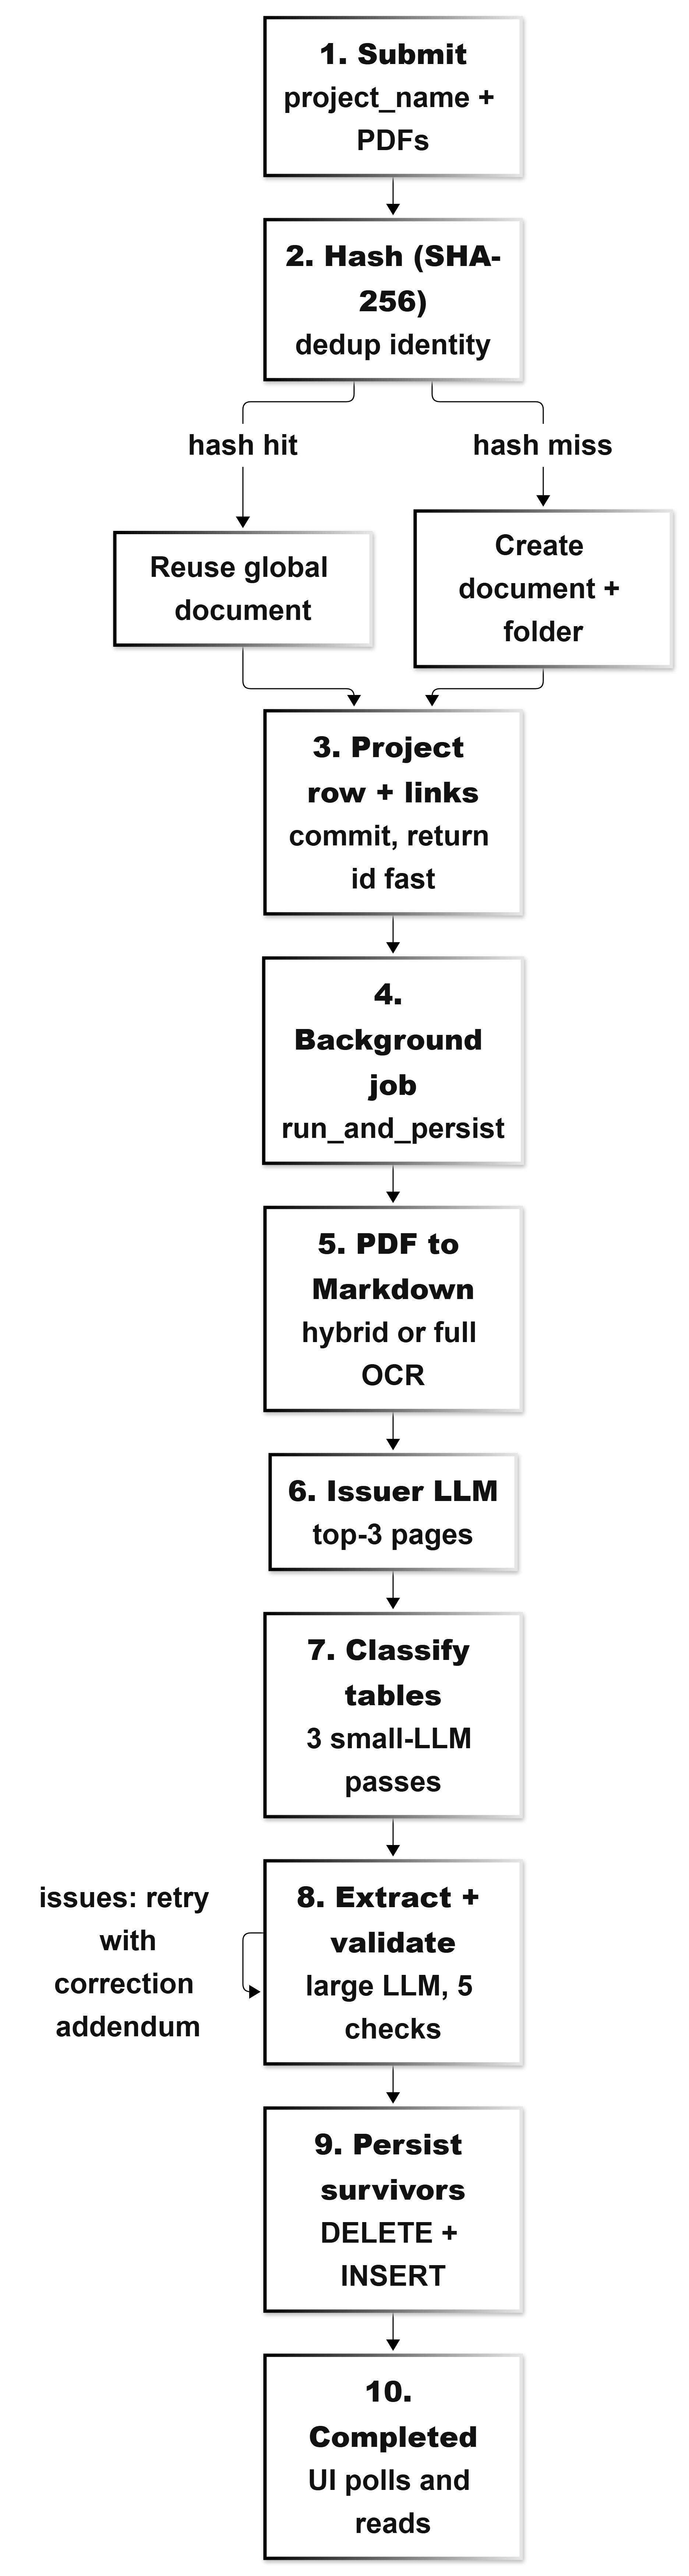
\includegraphics[width=\textwidth,height=0.85\textheight,keepaspectratio]{../diagrams/findoc_intelligence/01_flowchart_4-1-end-to-end-flow.png}
\caption{End-to-End Flow}
\label{fig:ch03_findoc_data_extraction-01-flowchart-4-1-end-to-end-flow}
\end{figure}

\speaker{Interviewer}{Why return before the extraction completes? This is a small system. Would synchronous processing not be simpler?}

\speaker{Candidate}{The service is small, but PDF conversion, OCR, several LLM calls, and retry loops can take minutes. A synchronous request risks proxy timeouts and poor user experience. Fast acceptance also gives the user a project ID immediately. The UI can poll a simple status endpoint while the background task works.}

\speaker{Interviewer}{Is \texttt{BackgroundTasks} a durable job queue?}

\speaker{Candidate}{No. It is an in-process background task. If the process crashes, the job can be lost. That is acceptable for the first version if we document the trade-off. At higher scale, I would move the work to a durable queue such as Celery, RQ, or a cloud-native job system.}

\speaker{Interviewer}{Let us go deeper. How do you validate uploaded PDFs and deduplicate them?}

\medskip\hrule\medskip
\section{Input Processing in Depth}
\label{sec:ch03_findoc_data_extraction-5-input-processing-in-depth}

\subsection{File Validation}

\speaker{Interviewer}{Walk me through file validation.}

\speaker{Candidate}{The service reads the uploaded bytes and checks the content signature. A valid PDF should begin with \texttt{\%PDF-}. XBRL is rejected based on its extension or known markers in the first few kilobytes. Any other unsupported input should raise an unsupported-document error.}

\speakcont{The file is then hashed with SHA-256. The hash is the global identity key. This means two uploads with identical bytes resolve to the same document row and storage folder, even if their filenames differ.}

\speaker{Interviewer}{Why hash the bytes instead of using the filename?}

\speaker{Candidate}{Filenames are not stable identities. Users can rename the same report or upload different content under the same name. Content hashing gives deterministic deduplication and protects against accidental replacement.}

\speaker{Interviewer}{How do you handle text PDFs versus scanned pages?}

\subsection{Text and Scanned PDFs}

\speaker{Interviewer}{How do you decide whether to use normal extraction or OCR?}

\speaker{Candidate}{The classifier uses PyMuPDF heuristics. It checks image dominance and whether pages contain enough text. A document is considered scanned when enough pages are image-dominant or when there is no usable text layer.}

\speakcont{For normal documents, the hybrid extractor processes each page. Pages containing tables or sufficient image area can be sent through OCR, while ordinary text pages can be converted with \texttt{pymupdf4llm}. For scanned documents, full-document OCR is used.}

\speaker{Interviewer}{Why not always use OCR?}

\speaker{Candidate}{OCR is slower and may introduce transcription errors in text that was already available accurately. Using OCR selectively reduces cost and latency while still handling image-heavy tables.}

\speaker{Interviewer}{What if there is no extractable text and OCR also fails?}

\speaker{Candidate}{The pipeline should return a diagnostic and skip downstream extraction for that document. It must not manufacture an empty success that looks like a correctly understood report.}

\speaker{Interviewer}{Why convert the PDF into Markdown before table extraction?}

\subsection{Markdown as the Internal Contract}

\speaker{Interviewer}{Why convert the PDF into Markdown rather than sending the raw PDF to the LLM?}

\speaker{Candidate}{The extraction pipeline is table-oriented. Markdown gives us page boundaries, headings, captions, and HTML table structure in a format that the table agents can inspect consistently. It also makes artifacts easy to save and debug.}

\speakcont{Every page is represented using a heading such as \texttt{\#\# Page 12}, and tables are represented as HTML. That lets downstream code identify the source page and lets the LLM see rows and columns without dealing with raw PDF bytes.}

\speaker{Interviewer}{What happens if OCR creates malformed HTML tables?}

\speaker{Candidate}{The table post-processor repairs common OCR problems, such as merged cells separated by pipe characters, inconsistent \texttt{rowspan} and \texttt{colspan}, and missing grid cells. It attempts to produce a rectangular table before the LLM sees it.}

\speaker{Candidate}{The Markdown contract is clear. Shall we discuss issuer detection and table discovery?}

\medskip\hrule\medskip
\section{Metadata and Table Discovery}
\label{sec:ch03_findoc_data_extraction-6-metadata-and-table-discovery}

\subsection{Issuer Metadata}

\speaker{Interviewer}{How does the system determine the company name and reporting period?}

\speaker{Candidate}{First, the document pages are loaded into a lightweight page index. An embedding search is performed using a query such as ``company name annual report financial year reporting currency document type.'' The top three relevant pages are assembled into an evidence block. A small LLM then returns JSON containing issuer, period, currency, and document type.}

\speaker{Interviewer}{Why retrieve only the top three pages?}

\speaker{Candidate}{Issuer metadata is usually concentrated on the cover, reporting-period page, or document information page. Retrieving a small amount of targeted evidence keeps the call cheaper and reduces irrelevant context. If metadata is not found, the detector fails softly and stores null values.}

\speaker{Interviewer}{Is this web search?}

\speaker{Candidate}{No. It searches the uploaded document's own indexed pages. This version would have no internet or news module, no DuckDuckGo integration, no yfinance integration, and no sentiment model.}

\speaker{Interviewer}{Once issuer metadata is set, how do you locate candidate tables without an LLM?}

\subsection{Finding Tables Without the LLM}

\speaker{Interviewer}{How do you find candidate tables?}

\speaker{Candidate}{The table finder parses the Markdown and tracks HTML table boundaries. It also tracks nearby headings, page numbers, captions, and outer scale annotations such as ``in millions.'' This step does not call the LLM.}

\speakcont{The output is a list of statement candidates. Each candidate includes the HTML table, page, nearby headings, caption, and scale context.}

\speaker{Interviewer}{Why not ask the LLM to find tables as well?}

\speaker{Candidate}{Table discovery is a structural task. Deterministic parsing is cheaper, repeatable, and easier to test. The LLM should focus on semantic decisions that are harder to encode with simple rules.}

\speaker{Interviewer}{With candidates found, how do you filter for analyst-relevant tables?}

\subsection{Relevance Filtering}

\speaker{Interviewer}{What does the first LLM table agent do?}

\speaker{Candidate}{It decides whether a candidate table contains an analyst-useful datapoint. Relevant examples include income statements, balance sheets, cash-flow statements, segment financials, loans, deposits, expenses, capital, risk-weighted assets, maturity breakdowns, KPIs, ratios, ratings, and share counts. Narrative-only pages, glossaries, and contact tables are dropped.}

\speakcont{The output is a structured object with \texttt{relevant} and a short \texttt{reason}.}

\speaker{Interviewer}{What happens if the LLM call fails?}

\speaker{Candidate}{The table would be dropped under fail-soft behavior. In a later production hardening step, I would record the failure reason and consider retrying transient model errors separately from a genuine ``not relevant'' decision.}

\speaker{Candidate}{Relevance filtering is clear. Shall we move to statement classification and consolidation?}

\medskip\hrule\medskip
\section{Classification and Consolidation}
\label{sec:ch03_findoc_data_extraction-7-classification-and-consolidation}

\subsection{Statement Classification}

\speaker{Interviewer}{How are relevant tables classified?}

\speaker{Candidate}{A small LLM assigns each table to one of five buckets:}

\begin{itemize}[leftmargin=\speakwid]
\item \texttt{balance\_sheet}.
\item \texttt{income\_statement}.
\item \texttt{cash\_flow}.
\item \texttt{changes\_in\_equity}.
\item \texttt{other}.
\end{itemize}
\speakcont{It also indicates whether the table is a breakdown and, if so, what it breaks down. The classifier should read row labels rather than relying only on page headings. For example, capital, RWA, and MREL tables are treated as balance-sheet-related, while KPI or ratio tables are kept under \texttt{other}.}

\speaker{Interviewer}{Why keep KPIs and ratios if the system does not calculate ratios?}

\speaker{Candidate}{They may be valuable reported datapoints. The system should extract what the document explicitly reports without pretending to calculate anything that is not built.}

\speaker{Interviewer}{How do you select consolidated columns and handle segment context?}

\subsection{Consolidated Column Selection}

\speaker{Interviewer}{Explain the consolidation step carefully.}

\speaker{Candidate}{Financial reports often show multiple columns such as Group, Bank, Company, Parent, standalone, segment, current year, prior year, and change percentage. The consolidation agent receives numbered headers and determines which columns represent the intended consolidated view.}

\speakcont{Group, Consolidated, Holding, or an unqualified total generally maps to consolidated. Bank, Company, Parent, or Standalone generally maps to unconsolidated. Change, variance, percentage-difference, and similar columns are skipped. If the table is clearly a segment table, the agent records a segment ID and treats the segment columns as consolidated within that segment.}

\speaker{Interviewer}{Why not extract every numeric column and let the user decide later?}

\speaker{Candidate}{That would create duplicate or misleading facts. For a consolidated financial analysis, extracting parent-only and group figures as if they represented the same entity can corrupt downstream use. Explicit column selection creates a cleaner contract.}

\speaker{Interviewer}{What if no consolidated column exists?}

\speaker{Candidate}{If there is a valid segment context, the table can still be retained with a segment ID. Otherwise, if there are no usable consolidated columns, the table is skipped under the consolidation rule.}

\speaker{Interviewer}{Now for the core step --- how do you extract flattened line items?}

\medskip\hrule\medskip
\section{Line-Item Extraction}
\label{sec:ch03_findoc_data_extraction-8-line-item-extraction}

\speaker{Interviewer}{Now explain the most important part: how do you extract line items?}

\speaker{Candidate}{The large extraction model receives the candidate summary, statement type, segment information, breakdown metadata, columns to keep, scale context, and the HTML table. It returns structured line items. Each line item has a label, section path, and one or more numeric cells.}

\speakcont{Each cell stores:}

\begin{itemize}[leftmargin=\speakwid]
\item Period end date.
\item Period type such as point, 3M, 6M, 9M, or 12M.
\item Segment ID when applicable.
\item Consolidation status.
\item Numeric value.
\item Currency.
\item Scale.
\item Raw text.
\item Source page or table reference.
\end{itemize}
\speaker{Interviewer}{Why retain both the parsed numeric value and raw text?}

\speaker{Candidate}{The numeric value supports querying and downstream computation. Raw text preserves what appeared in the document, including parentheses, currency symbols, commas, and footnote markers. If a reviewer questions a negative value or a scaling decision, raw text helps diagnose it.}

\speaker{Interviewer}{How do you handle parentheses?}

\speaker{Candidate}{A value such as \texttt{(123)} is converted to \texttt{-123}, while the raw token remains available. The validator later checks that the sign conversion is consistent.}

\speaker{Interviewer}{What columns should be skipped?}

\speaker{Candidate}{Variance columns should normally be excluded: Change, Difference, Variance, Amount change, percentage change, basis-point change, Increase, Decrease, versus, and similar labels. These are not independent financial statement values.}

\speaker{Interviewer}{What about a row with a label such as ``Revenue growth \%''?}

\speaker{Candidate}{If the table explicitly reports it as a KPI and the classifier keeps the table, it can be retained as a reported KPI. But the extraction prompt must distinguish a reported metric from a variance column and preserve the correct scale.}

\speaker{Interviewer}{How do you preserve hierarchy?}

\speaker{Candidate}{The line item is flat, but it carries a \texttt{section\_path}. For example, a line item may have \texttt{['Assets', 'Current assets']}. This preserves context without forcing every consumer to understand a nested tree structure.}

\speaker{Interviewer}{Why not store a nested JSON tree?}

\speaker{Candidate}{Flat records are simpler to query, compare, validate, and render. \texttt{section\_path} retains the hierarchy while keeping each numeric fact independently addressable.}
\speaker{Candidate}{Before we leave extraction, can I detail the flattening and context rules that determine what the analyst sees per cell?}
\speaker{Interviewer}{Yes, explain how raw cells become analyst-ready records.}
\speaker{Candidate}{Each extracted cell becomes one flat record with an ISO period end date and a period length in months, where 3M, 6M, 9M, and 12M map to 3, 6, 9, and 12, and a point-in-time balance-sheet row maps to no length. As examples, a third-quarter column maps to 3M and a full-year column maps to 12M. The record keeps a \texttt{source\_snippet} tag naming its page, a boolean consolidation flag, and page number, so the analyst can trace any number back to its table.}
\speakcont{Hierarchy is tracked with a section stack: a subheader is pushed when it appears, popped when a matching total or net line closes it, and conflicting headers are popped so the \texttt{section\_path} stays outermost-first. Probability-of-default band tables append the metric header to the label, so a band and its measure stay distinguishable. Currency and scale follow a precedence of row first, then subheader, then the outer annotation such as ``in millions,'' with per-row annotations such as a euro-billions marker, a percent sign, or a basis-points marker overriding the table default. The \texttt{unit} field is derived rather than left empty: percentage, thousands, millions, and billions pass through and anything else becomes absolute. When a cell has no currency, the detected issuer currency backfills it, which keeps multi-table documents comparable for the analyst instead of leaving blanks that look like missing data.}

\speaker{Interviewer}{How do you validate extracted values and retry when checks fail?}

\medskip\hrule\medskip
\section{Validation and Retry}
\label{sec:ch03_findoc_data_extraction-9-validation-and-retry}

\speaker{Interviewer}{How do you know the extracted values are reasonable?}

\speaker{Candidate}{After extraction, the pipeline aggregates values and runs deterministic validators. The checks I would include are:}

\begin{enumerate}[leftmargin=\speakwid]
\item Bracket-sign validation: parenthesized raw values should become negative.
\item Numeric-label validation: labels should not be bare numbers or numeric ranges.
\item Duplicate-value warning: identical values with different periods or segments may indicate a possible extraction issue.
\item Ambiguous-duplicate-label error: the same label, section, period, and segment should not have conflicting values.
\item Period-type mismatch: balance-sheet facts should be point-in-time, while flow statements should use 3M, 6M, 9M, or 12M periods.
\end{enumerate}
\speaker{Interviewer}{Can you add deterministic checks and what correctness gate on the LLM outputs would you propose, and why do they matter to the analyst?}
\speaker{Candidate}{They close the gap between ``the output parsed cleanly'' and ``the output is plausibly correct for analysis.'' The first additional check is currency-and-scale consistency. If one line item mixes currencies, or mixes a percentage scale with an absolute scale, the validator records an error. For the analyst this matters because a mixed-currency row or a 13.4 percent ratio stored as 13.4 million would silently corrupt any spreadsheet or downstream comparison. On failure the affected cells keep a \texttt{validation\_errors} entry, a correction note names the offending label and expected single currency and scale, and the extraction step retries with that note.}
\speakcont{The second additional check is the balance-sheet identity. When total assets, total liabilities, and total equity are all present for the same period, the validator compares assets against liabilities plus equity with a one-percent tolerance and records an error if they do not reconcile. For the analyst this mirrors the first thing a reviewer does with a balance sheet: confirm it balances. It catches misclassified totals, dropped signs, and scale slips. It only fires when all three totals are present, so partial extractions do not raise false alarms. Both checks feed the same correction-addendum retry loop as the other five.}
\speakcont{Above those deterministic rules sits a correctness-gate layer. It scores statement classification as a percent-correct against captions and headers, scores each extracted cell with a confidence for label, currency, scale, and plausibility, and provides an accounting-identity helper. Any cell with confidence below 0.50 is treated like a failed validation: it is listed with the other failures and its description is appended to the retry prompt. That way low-confidence LLM output gets a second chance with explicit guidance instead of passing silently into the analyst view.}
\speaker{Interviewer}{Are these checks supposed to prove that every number is correct?}

\speaker{Candidate}{No. They detect suspicious patterns and common extraction errors. They are quality controls, not a replacement for a labelled evaluation set or human review.}

\speaker{Interviewer}{What happens when validation finds an issue?}

\speaker{Candidate}{The system attributes the issue to the source table where possible and creates correction notes. On the next iteration, the extraction model receives those notes. Classification is not repeated. Only line-item extraction and aggregation run again.}

\speaker{Interviewer}{Why retry only the last part?}

\speaker{Candidate}{Earlier stages have already decided which tables are relevant and which columns should be retained. Repeating them would add cost and could introduce inconsistency. Retrying the extraction step directly targets the problem identified by validation.}

\speaker{Interviewer}{What happens after three attempts?}

\speaker{Candidate}{The final survivors are persisted, and each affected line item retains its validation errors. The project does not pretend that flagged values are perfect, but it also does not lose potentially useful data.}
\speaker{Candidate}{Since validation drives the retry, can I spell out exactly how failures are listed and fed back into the prompt?}
\speaker{Interviewer}{Yes, walk me through the failed-validation listing and the retry prompt.}
\speaker{Candidate}{Every surviving line item carries a \texttt{validation\_errors} list, where each entry names the check, a severity of warning or error, and a human-readable message. Per iteration the pipeline also writes an \texttt{extraction.json} and a \texttt{validation\_report.json} under the document prefix in S3 or ADLS, so the analyst or auditor can see which iteration raised what. The Documents tab surfaces a flagged-item count from those lists, which is how the business user decides what to trust and what to verify against the source page.}
\speakcont{For the retry, the pipeline maps each issue back to its source table through a page-to-table map and builds a correction addendum that tells the extraction model its previous output was validated and lists the specific issues found, one note per problem. Those notes are appended to the user message alongside the table HTML on the next attempt, so the large model sees both the original table and the exceptions it must fix. Classification stays frozen and only extraction plus aggregation re-run, up to three iterations. Confidence-gate failures below 0.50 travel the same path: their descriptions join the addendum. If issues remain after the third attempt, the records persist with their flags rather than being discarded, which preserves analyst access while keeping quality concerns visible.}

\speaker{Interviewer}{Can you show me the retry sequence across extraction and validation?}

\subsection{Retry Flow}

\begin{figure}[htbp]
\centering
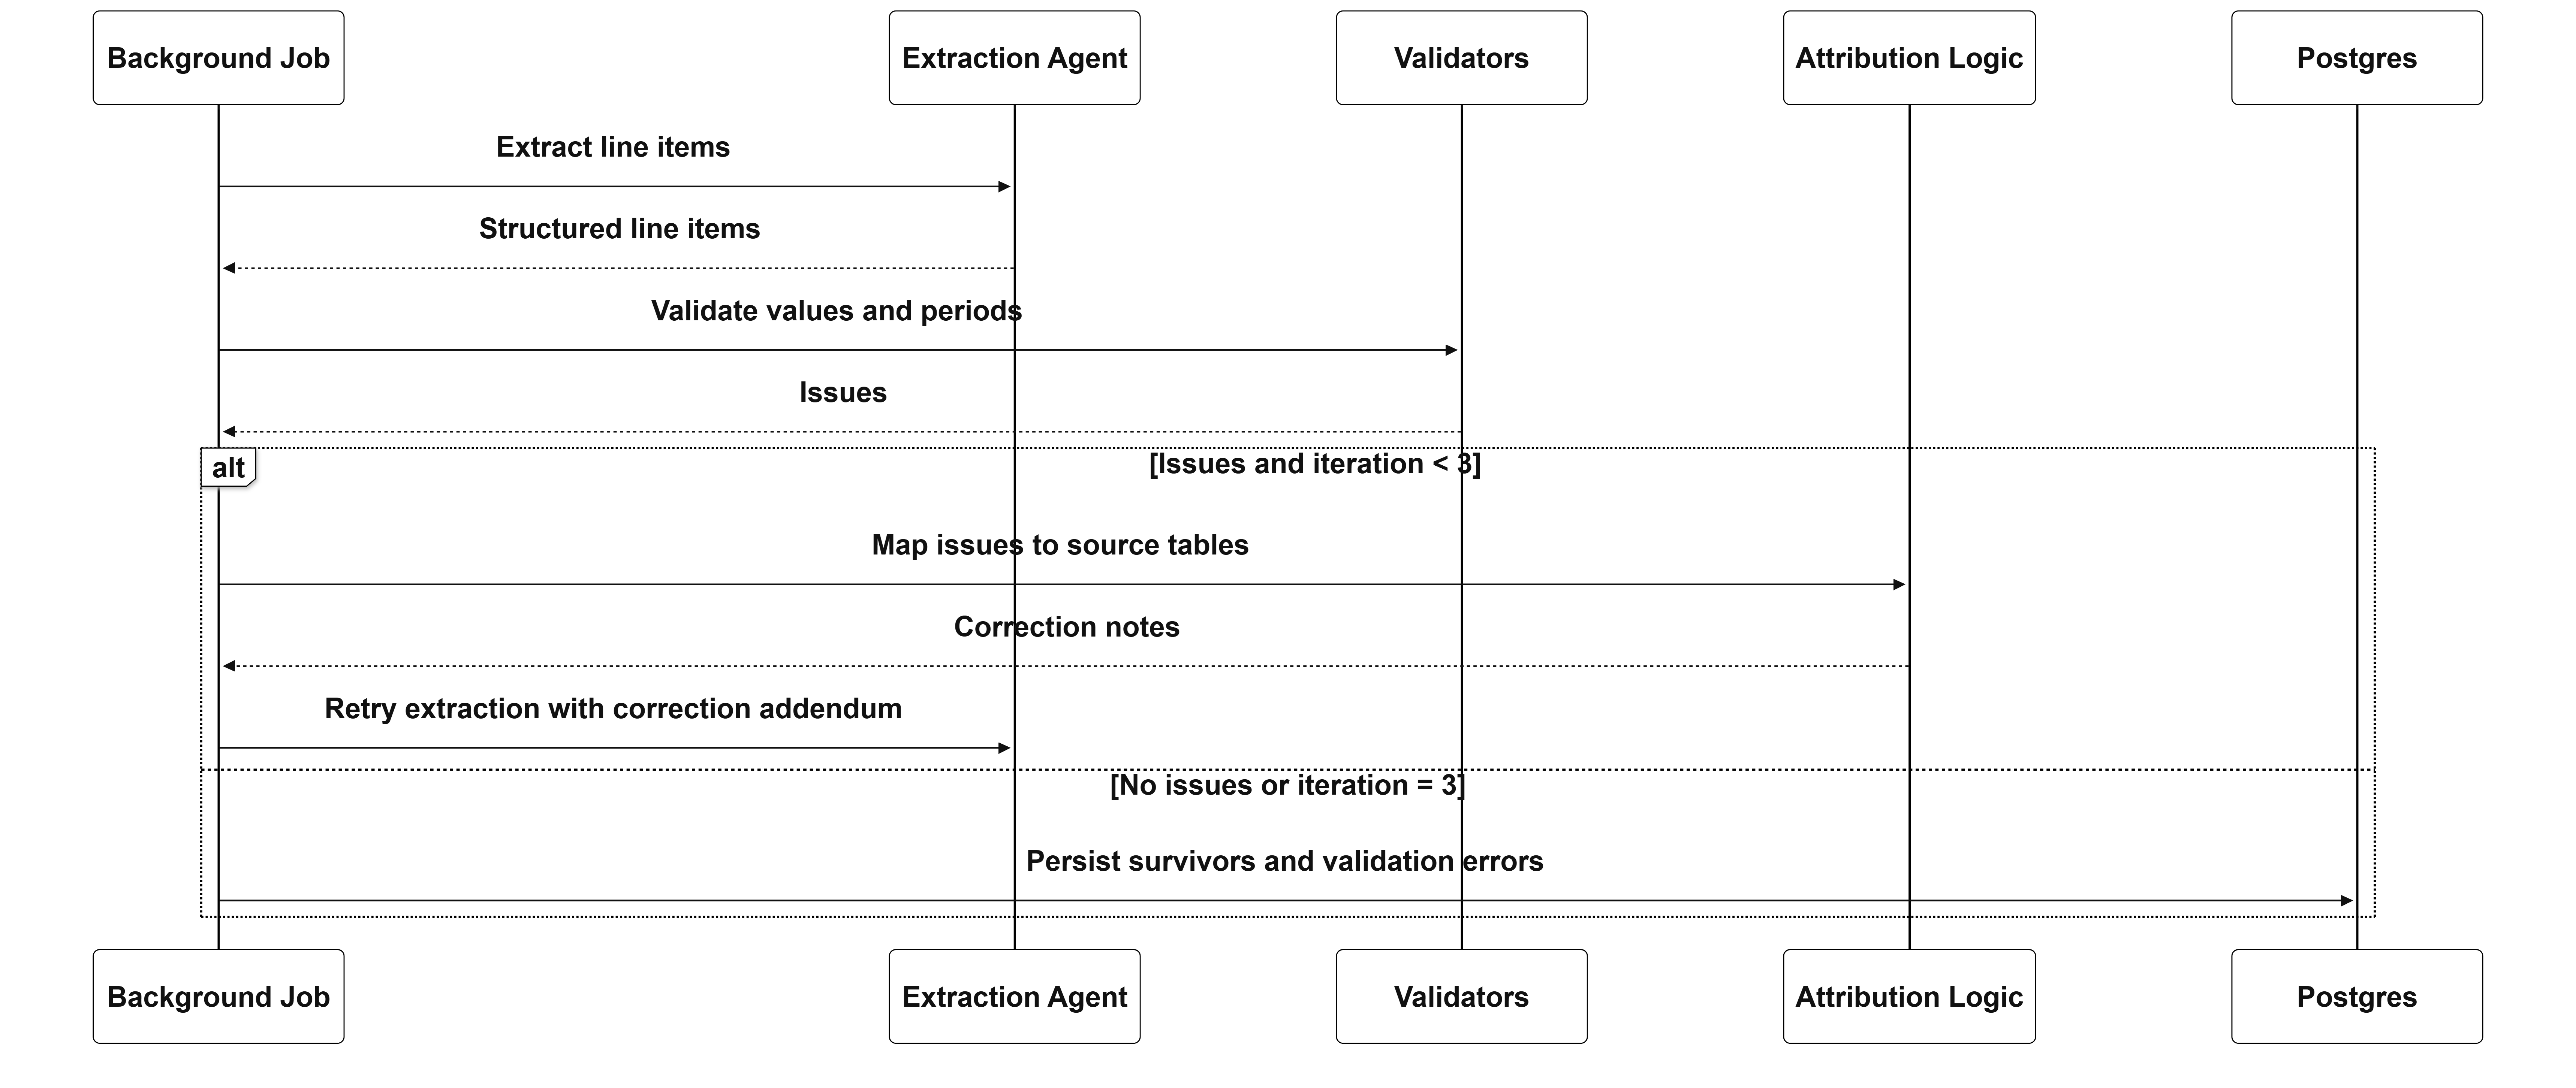
\includegraphics[width=\textwidth,height=0.85\textheight,keepaspectratio]{../diagrams/findoc_intelligence/02_sequenceDiagram_retry-flow.png}
\caption{Retry Flow}
\label{fig:ch03_findoc_data_extraction-02-sequencediagram-retry-flow}
\end{figure}

\speaker{Interviewer}{Let us turn to persistence. How do projects, documents, and line items map to Postgres and object storage?}

\medskip\hrule\medskip
\section{Data Modeling}
\label{sec:ch03_findoc_data_extraction-10-data-modeling}

\speaker{Interviewer}{Explain the database and storage design.}

\speaker{Candidate}{I would use four main Postgres tables:}

\begin{itemize}[leftmargin=\speakwid]
\item \texttt{projects} for one upload event and its overall processing status.
\item \texttt{documents} for globally deduplicated document identity and metadata.
\item \texttt{project\_documents} as the many-to-many-style association between projects and documents.
\item \texttt{line\_items} for flattened extracted financial facts.
\end{itemize}
\speakcont{Files and processing artifacts are stored in S3 or ADLS under a document-specific prefix. The PDF in object storage is authoritative. Markdown and per-iteration JSON artifacts are stored alongside it, and all reads use object-storage URIs.}

\speaker{Interviewer}{Why separate projects from globally deduplicated documents?}

\subsection{Why Separate Projects and Documents?}

\speaker{Interviewer}{Why not put the document directly inside the project table?}

\speaker{Candidate}{Because the same document may be uploaded in multiple projects. A project represents an upload event or analysis grouping, while a document represents unique file content. Global document identity lets us reuse the same document record and storage folder.}

\speaker{Interviewer}{What happens if the same PDF is uploaded with a different filename?}

\speaker{Candidate}{The SHA-256 hash resolves to the existing document. The first filename remains the stored filename. The second upload creates or reuses the project link but does not create a duplicate document.}

\speaker{Interviewer}{Does that mean line items belong to a project?}

\speaker{Candidate}{I would scope line items to the document, not directly to the project. This means reprocessing a globally shared document replaces its line items. That is a meaningful trade-off: if different projects require different extraction settings, the model would need project-scoped document versions in a future design.}

\speaker{Interviewer}{Can you show the entity relationships?}

\subsection{Entity Relationship Diagram}

\begin{figure}[htbp]
\centering
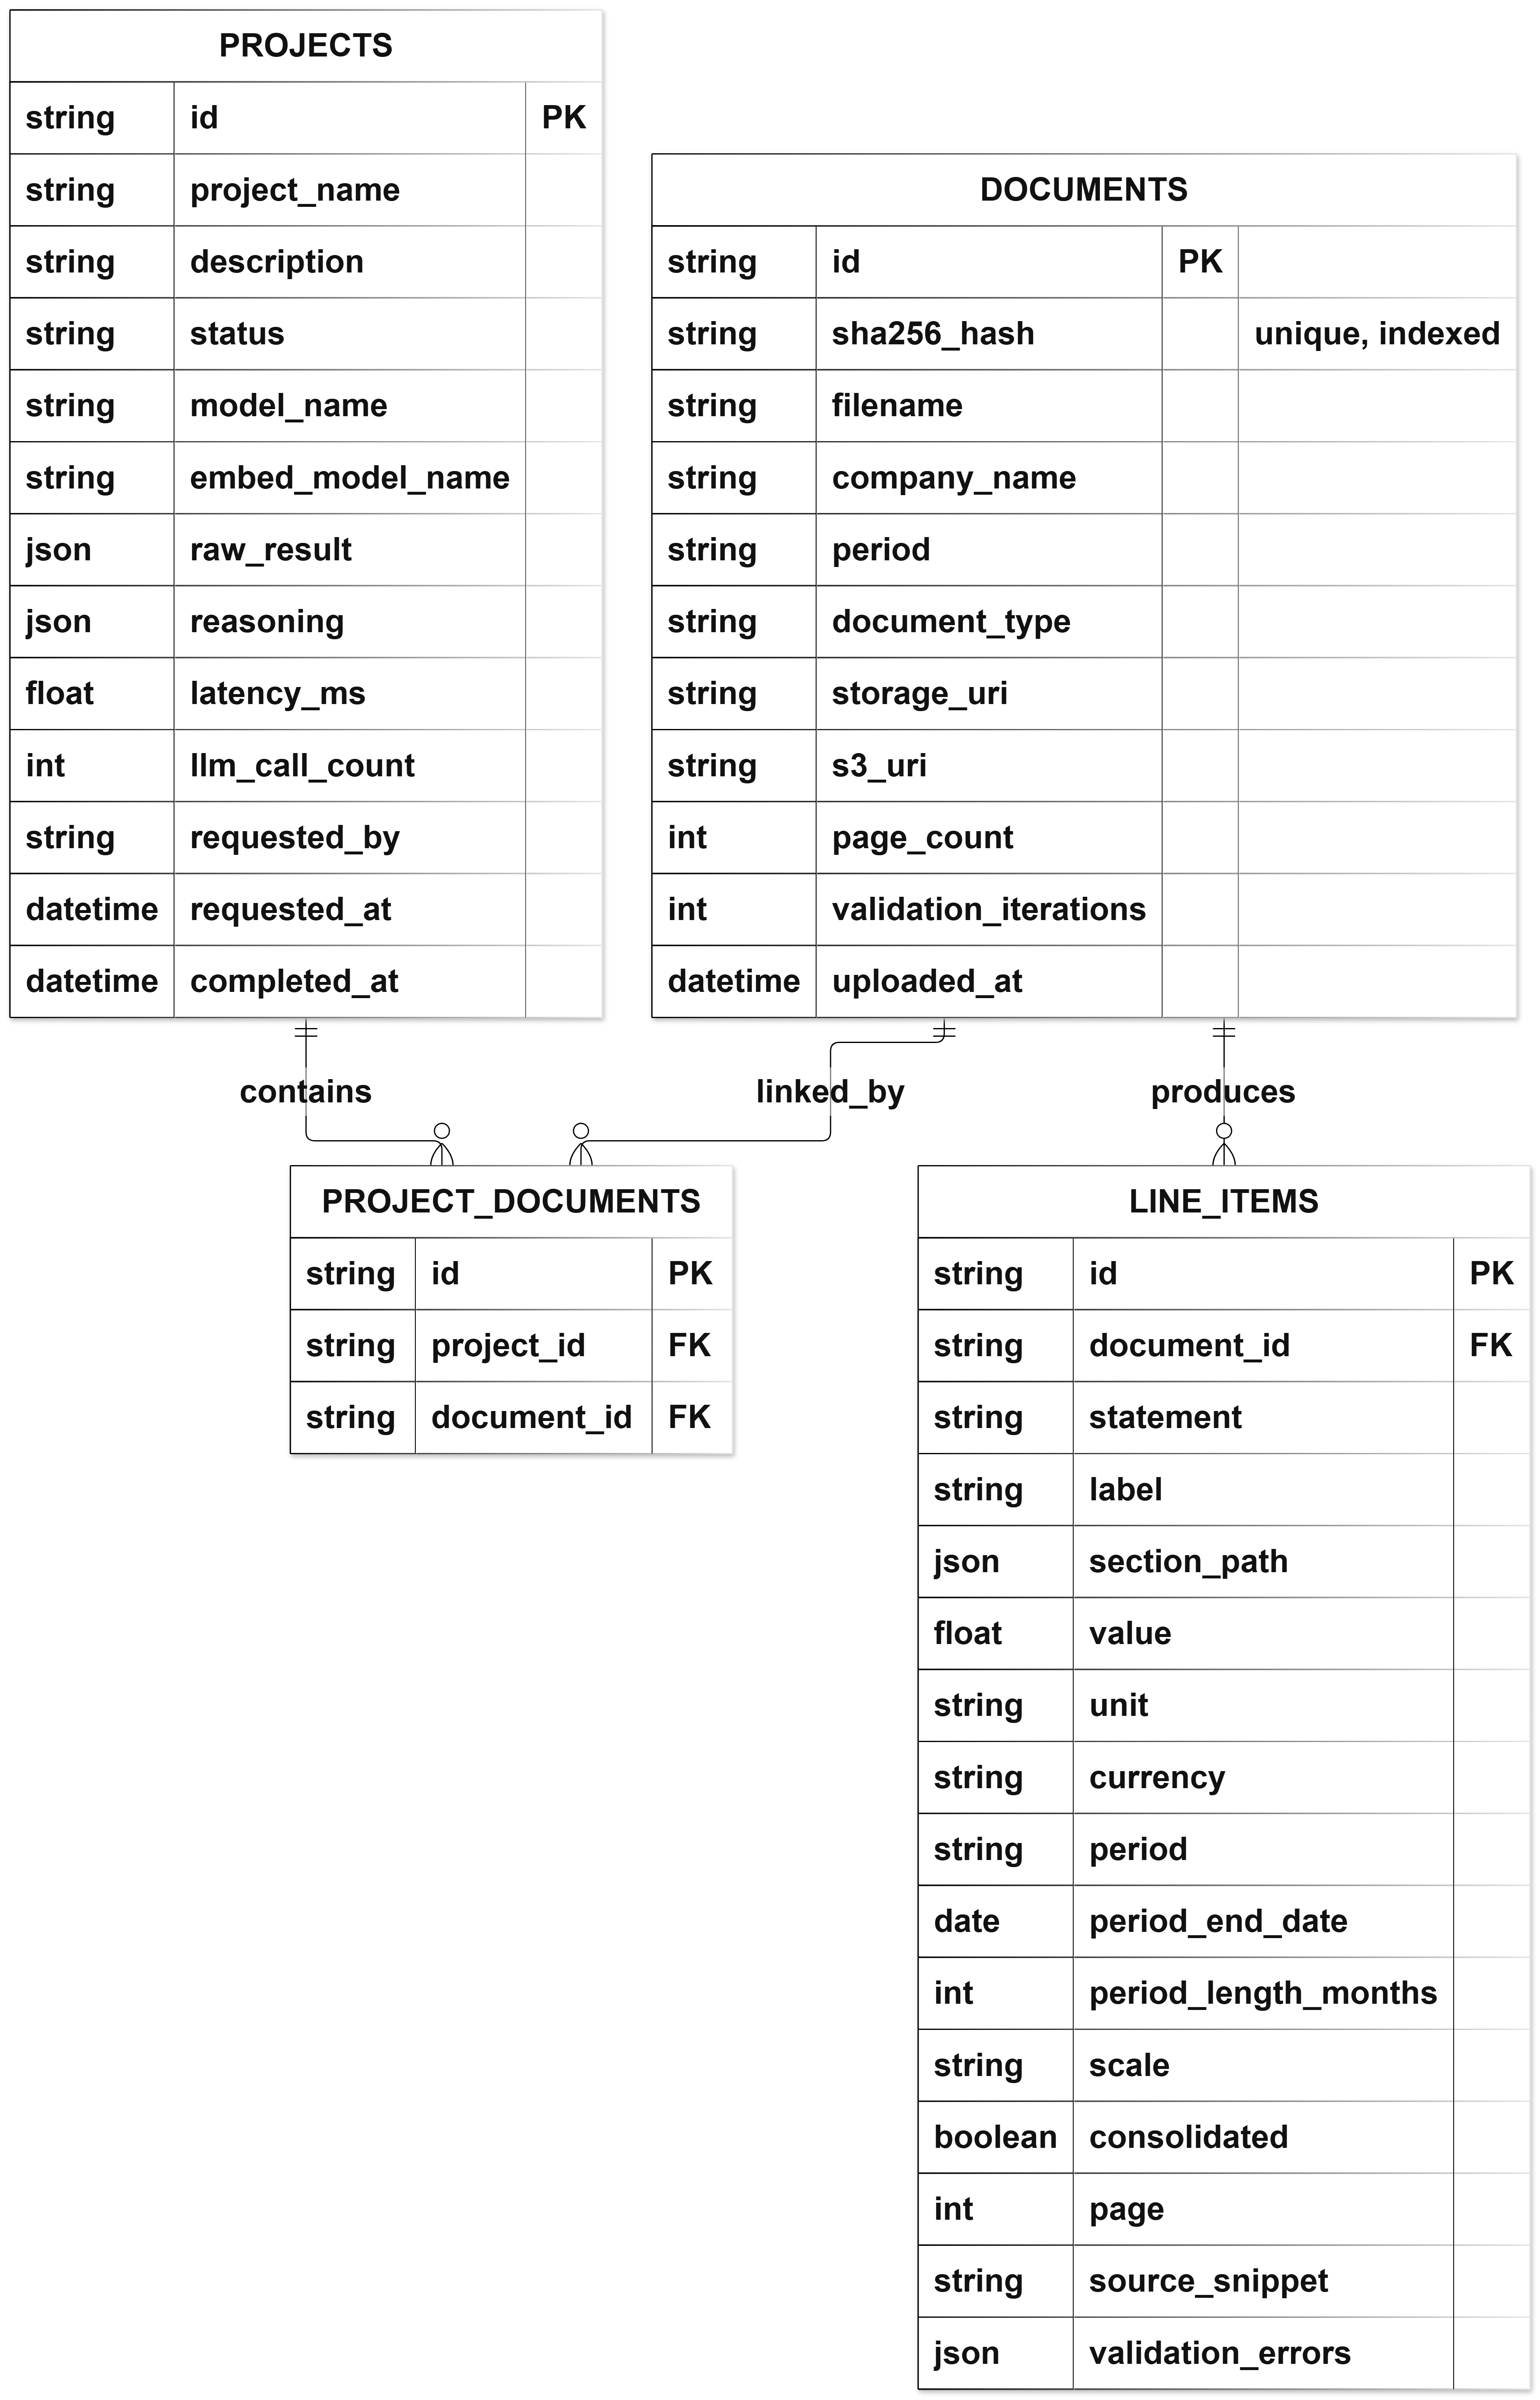
\includegraphics[width=\textwidth,height=0.85\textheight,keepaspectratio]{../diagrams/findoc_intelligence/03_erDiagram_10-2-entity-relationship-diagram.png}
\caption{Entity Relationship Diagram}
\label{fig:ch03_findoc_data_extraction-03-erdiagram-10-2-entity-relationship-diagram}
\end{figure}

\speaker{Interviewer}{What are the key columns and purposes for each table?}

\subsection{Data Model Table}

\begin{xltabular}{\textwidth}{>{\raggedright\arraybackslash}X >{\raggedright\arraybackslash}X >{\raggedright\arraybackslash}X >{\raggedright\arraybackslash}X}
\caption{Data Model Table}\label{tab:ch03_findoc_data_extraction-10-3-data-model-table-1}\\
\hline
\textbf{Entity} & \textbf{Important columns} & \textbf{Relationship} & \textbf{Purpose} \\
\hline
\endfirsthead
\caption[]{Data Model Table (continued)}\\
\hline
\textbf{Entity} & \textbf{Important columns} & \textbf{Relationship} & \textbf{Purpose} \\
\hline
\endhead
\texttt{projects} & \texttt{id}, \texttt{project\_name}, \texttt{status}, \texttt{raw\_result}, \texttt{latency\_ms}, \texttt{llm\_call\_count} & One project has many project-document links & Represents an upload event and processing lifecycle \\
\texttt{documents} & \texttt{id}, \texttt{sha256\_hash}, \texttt{filename}, \texttt{company\_name}, \texttt{period}, \texttt{document\_type}, \texttt{storage\_uri} & One document can be linked to many projects & Global content identity and document metadata \\
\texttt{project\_documents} & \texttt{project\_id}, \texttt{document\_id} & Joins projects and documents & Connects an upload event to its files \\
\texttt{line\_items} & \texttt{document\_id}, \texttt{statement}, \texttt{label}, \texttt{section\_path}, \texttt{value}, \texttt{period}, \texttt{page}, \texttt{validation\_errors} & One document has many line items & Stores flattened extracted financial facts \\
\hline
\end{xltabular}
\speaker{Candidate}{The summary table above shows the core columns, so can I record the full column set the analyst and operator depend on?}
\speaker{Interviewer}{Yes, give me the complete column picture and why each addition matters.}
\speaker{Candidate}{On \texttt{projects}, beyond name, status, raw result, latency, and call count, I would persist the chat model name, the embedding model name, and a reasoning payload, plus description, a free-text requester, request time, and completion time. For the business this records which model produced which project and when, which supports cost tracking, reproducibility, and audit. On \texttt{documents}, beyond identity hash, filename, company, period, type, and storage URI, I would persist an S3 or ADLS mirror URI used as fallback storage location, a page count from the PDF parser, an upload timestamp, and a validation-iterations count from 1 to 3. The iteration count tells the analyst how hard the pipeline worked on that document.}
\speakcont{On \texttt{line\_items}, I would persist document reference, statement bucket, verbatim label, section path, signed value, unit, currency, ISO period string, period end date, period length in months, scale, consolidation flag, page, source snippet page tag, and the surviving validation-errors list. The unit, currency, scale, and period-date columns are what let the analyst compare values across periods and documents without guessing scale, while the source snippet and page preserve lineage to the original table. I would keep primary storage URIs preferring the S3 or ADLS location as fallback so reads survive a move off any single machine.}
\speaker{Interviewer}{Which joins power the Documents tab and project browsing?}

\subsection{Join Examples}

\begin{xltabular}{\textwidth}{>{\raggedright\arraybackslash}X >{\raggedright\arraybackslash}X >{\raggedright\arraybackslash}X >{\raggedright\arraybackslash}X}
\caption{Join Examples}\label{tab:ch03_findoc_data_extraction-10-4-join-examples-2}\\
\hline
\textbf{From} & \textbf{To} & \textbf{Join condition} & \textbf{Why it matters} \\
\hline
\endfirsthead
\caption[]{Join Examples (continued)}\\
\hline
\textbf{From} & \textbf{To} & \textbf{Join condition} & \textbf{Why it matters} \\
\hline
\endhead
\texttt{projects} & \texttt{project\_documents} & \texttt{projects.id = project\_documents.project\_id} & Find documents uploaded in a project \\
\texttt{project\_documents} & \texttt{documents} & \texttt{project\_documents.document\_id = documents.id} & Load document metadata and storage location \\
\texttt{documents} & \texttt{line\_items} & \texttt{documents.id = line\_items.document\_id} & Load extracted facts for one document \\
\texttt{projects} & \texttt{documents} & \texttt{projects.id = project\_documents.project\_id} and \texttt{project\_documents.document\_id = documents.id} & Browse all documents belonging to a project \\
\hline
\end{xltabular}

\speaker{Interviewer}{Why store both normalized columns and a JSON result on the project?}

\speaker{Candidate}{Normalized \texttt{line\_items} make filtering, counting, and rendering practical. \texttt{raw\_result} preserves a compact document-level summary and diagnostics. The hybrid approach is more useful than storing everything in one large JSON field.}

\speaker{Candidate}{The data model is clear. Shall we define the API contract for uploads and retrieval?}

\medskip\hrule\medskip
\section{API Design}
\label{sec:ch03_findoc_data_extraction-11-api-design}

\speaker{Interviewer}{Can you describe the API contract?}

\speaker{Candidate}{The main endpoints are intentionally small.}

\begin{xltabular}{\textwidth}{>{\raggedright\arraybackslash}X >{\raggedright\arraybackslash}X >{\raggedright\arraybackslash}X}
\caption{API Design}\label{tab:ch03_findoc_data_extraction-11-api-design-3}\\
\hline
\textbf{Method} & \textbf{Endpoint} & \textbf{Purpose} \\
\hline
\endfirsthead
\caption[]{API Design (continued)}\\
\hline
\textbf{Method} & \textbf{Endpoint} & \textbf{Purpose} \\
\hline
\endhead
\texttt{GET} & \texttt{/} & Serve the web UI \\
\texttt{GET} & \texttt{/health} & Health check for deployment probes \\
\texttt{POST} & \texttt{/projects} & Accept project name, description, and one or more PDFs \\
\texttt{GET} & \texttt{/projects/\{id\}} & Return project details and per-document counts \\
\texttt{GET} & \texttt{/projects/\{id\}/status} & Return processing status and simple progress \\
\texttt{GET} & \texttt{/documents} & List documents for the Documents tab \\
\texttt{GET} & \texttt{/documents/\{id\}} & Return document metadata and grouped line items \\
\texttt{GET} & \texttt{/documents/\{id\}/file} & Serve the original PDF inline \\
\hline
\end{xltabular}


\begin{figure}[htbp]
\centering
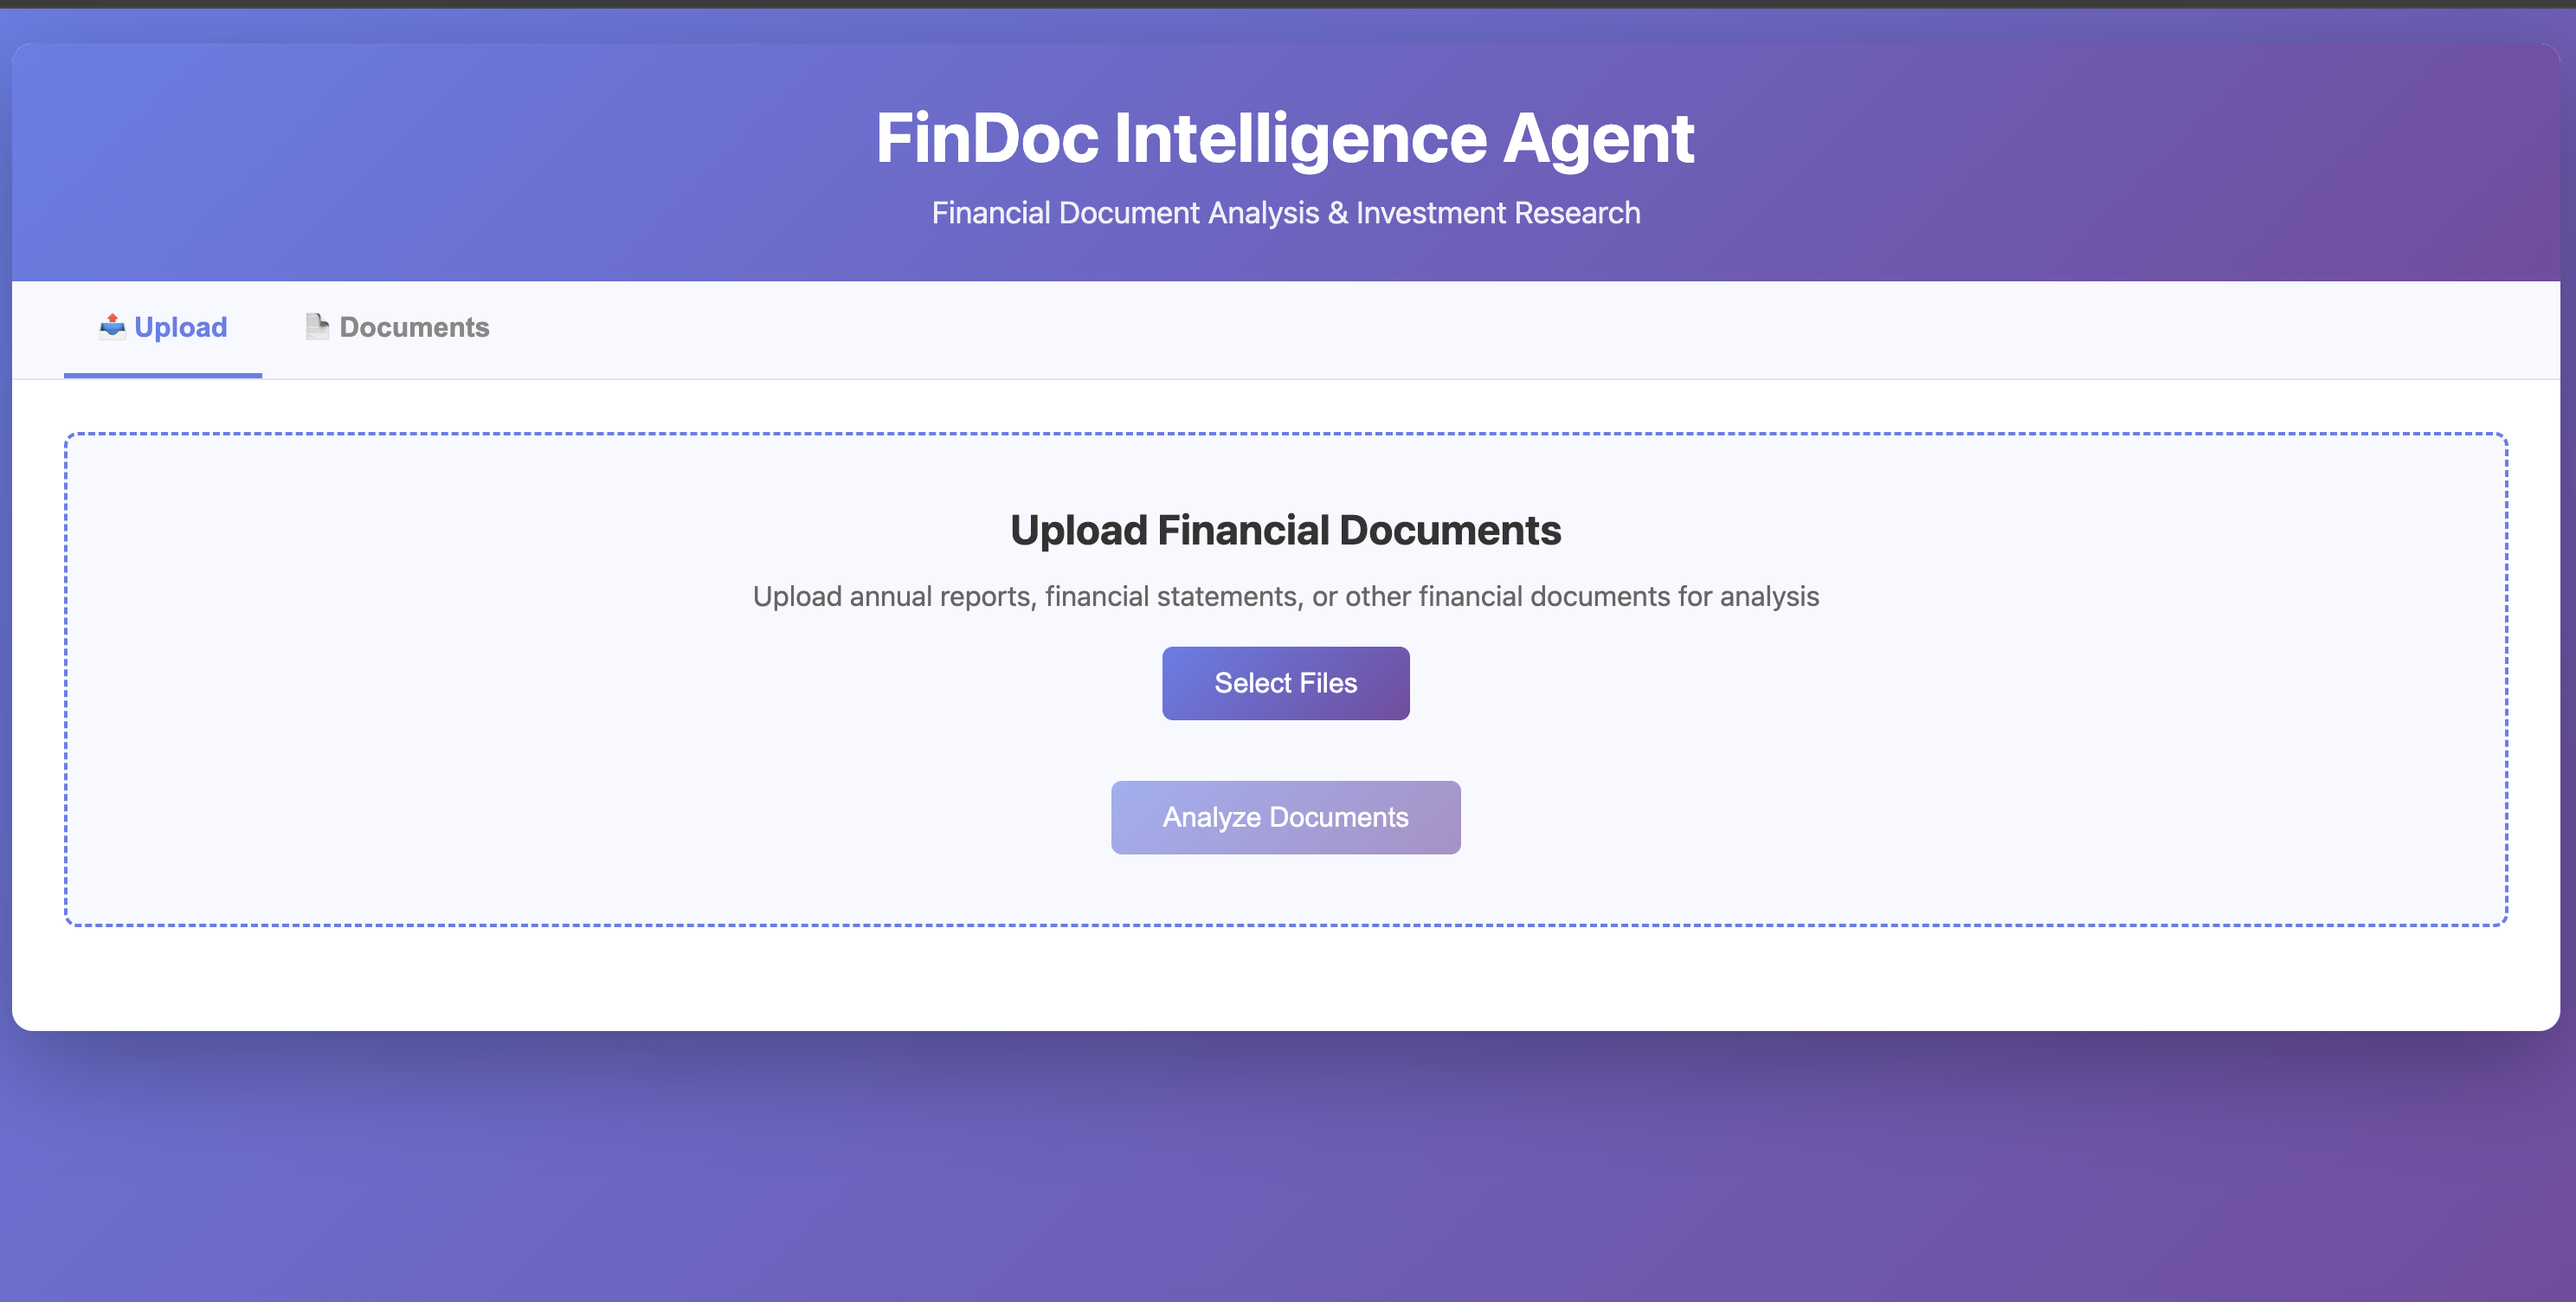
\includegraphics[width=\textwidth,height=0.85\textheight,keepaspectratio]{../diagrams/findoc_intelligence/screen_11_upload.png}
\caption{Upload view served by \texttt{GET /}: submit project details and PDFs for a new project.}
\label{fig:ch03_findoc_data_extraction-screen-11-upload}
\end{figure}

\speaker{Interviewer}{What does \texttt{POST /projects} do synchronously?}

\speaker{Candidate}{It reads the uploaded bytes, validates the document identity, hashes each file, resolves or inserts document rows, saves the PDFs, creates the project and link rows, commits them, schedules \texttt{run\_and\_persist}, and returns the project ID with status \texttt{processing}.}

\speaker{Interviewer}{What does it not do?}

\speaker{Candidate}{It does not perform OCR, table extraction, LLM classification, validation, or final persistence of line items before returning. Those happen in the background.}

\speaker{Interviewer}{How does the UI know the job is finished?}

\speaker{Candidate}{It polls \texttt{/projects/\{id\}/status}. The current status is stored in Postgres. The UI then calls the project or document detail endpoint to load final results.}


\begin{figure}[htbp]
\centering
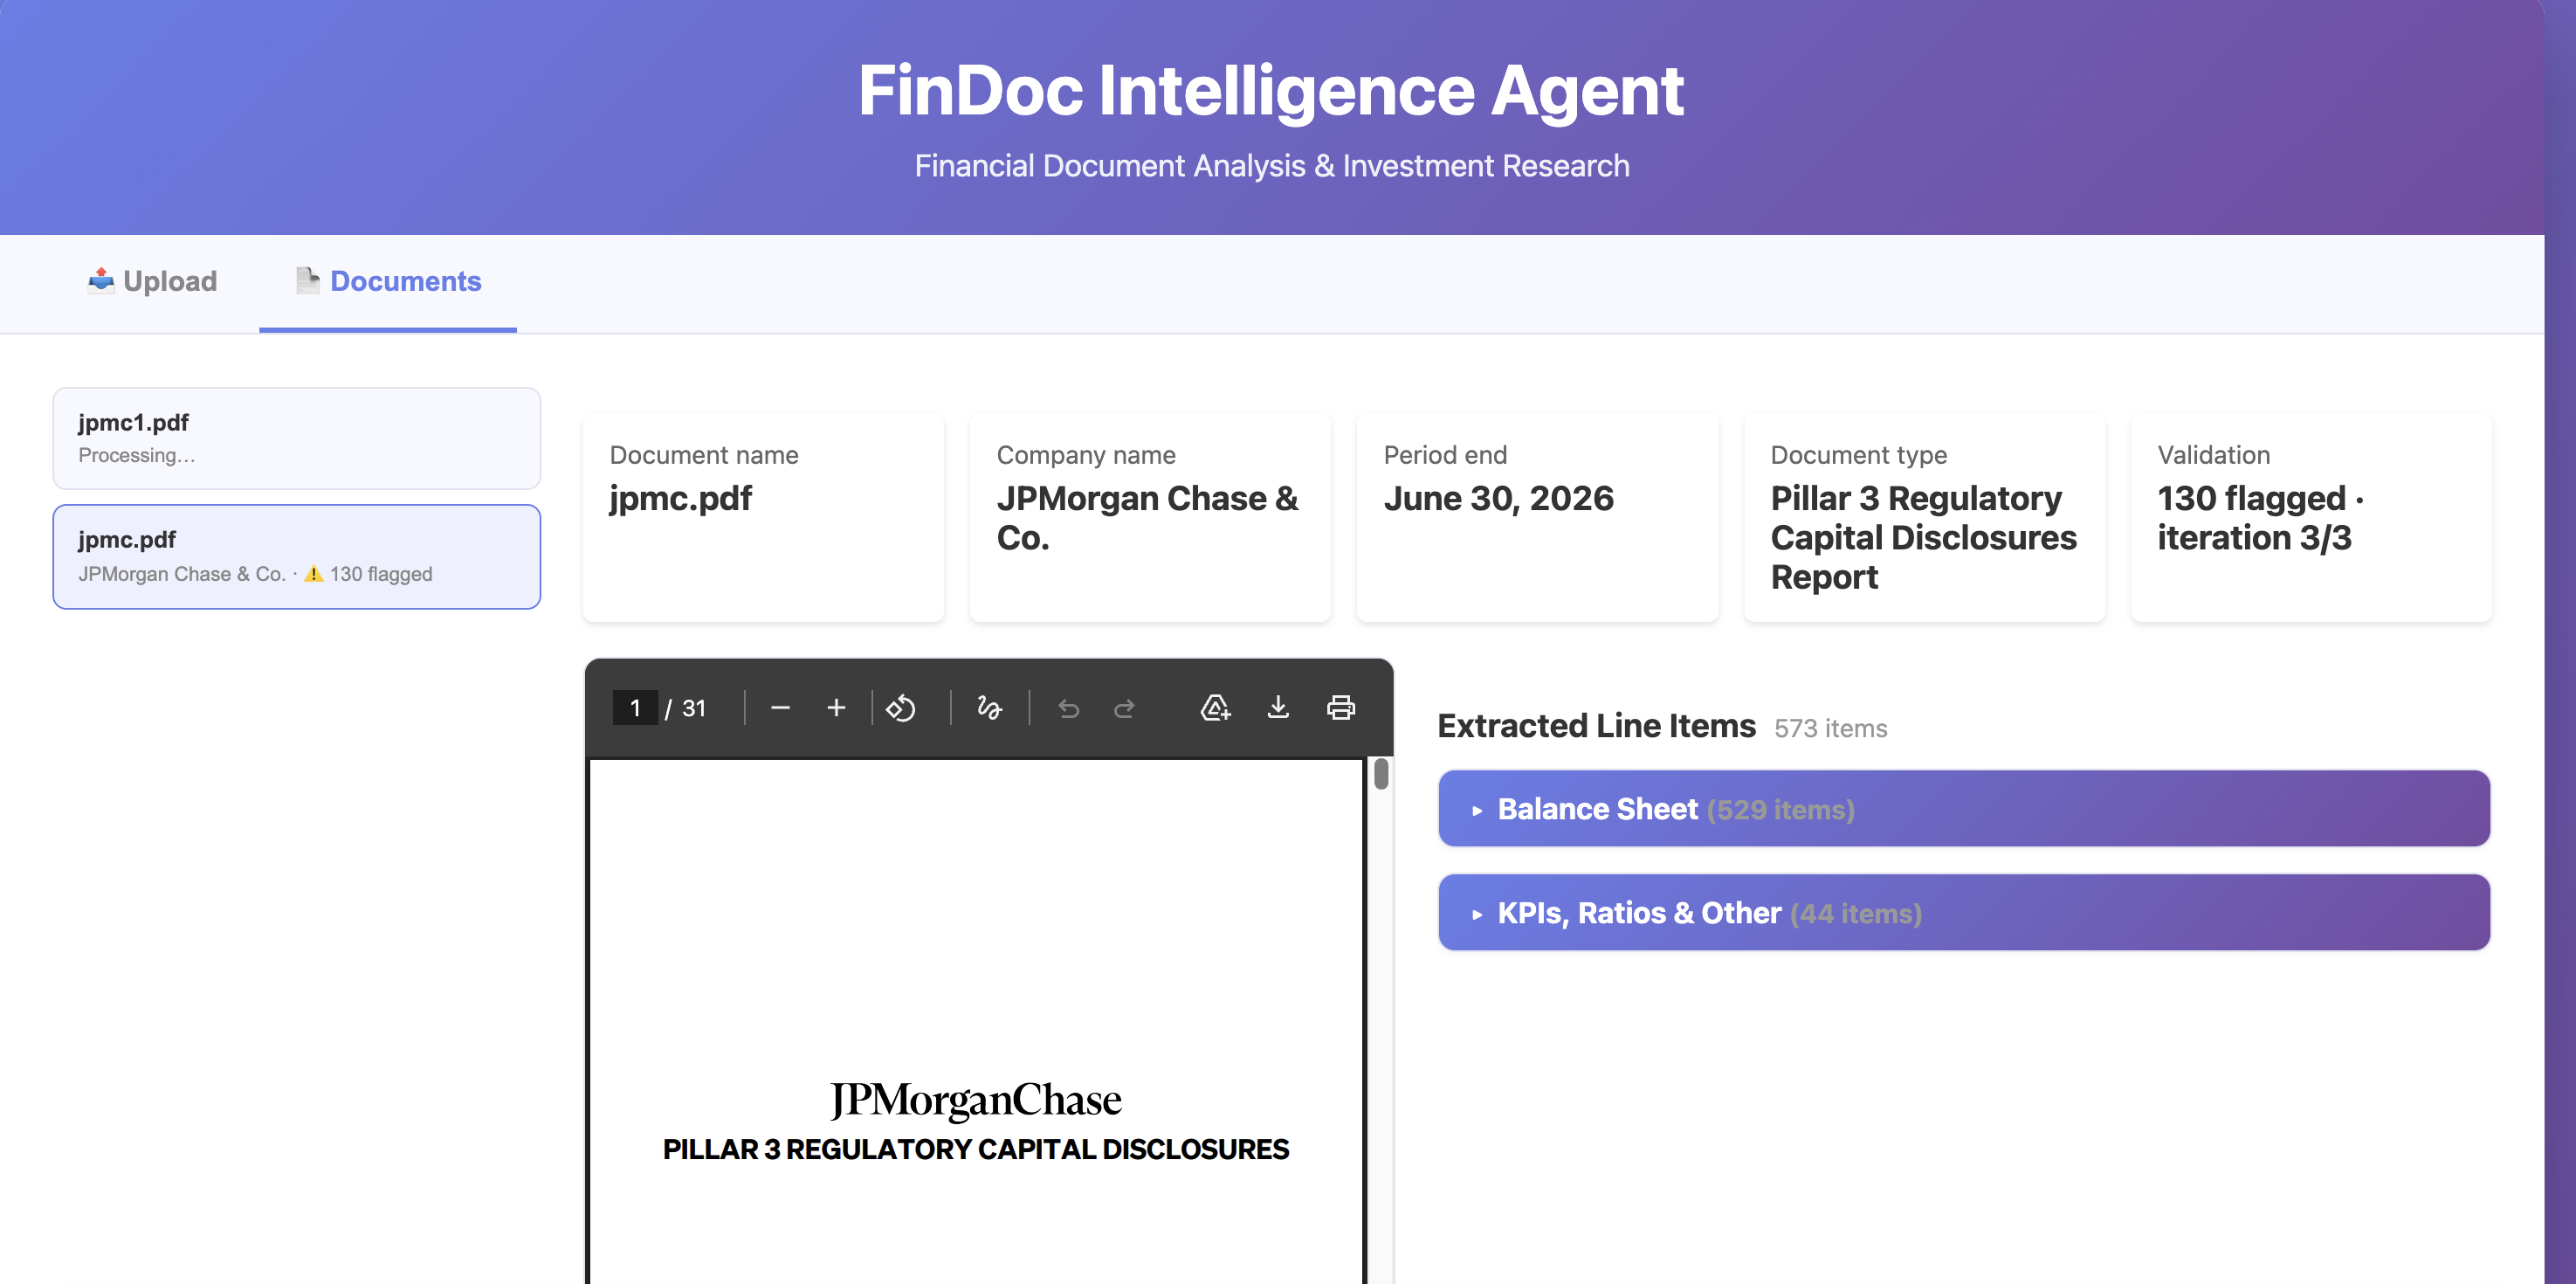
\includegraphics[width=\textwidth,height=0.85\textheight,keepaspectratio]{../diagrams/findoc_intelligence/screen_11_documents.png}
\caption{Documents tab backed by \texttt{GET /documents}: per-document metadata with grouped extracted line items.}
\label{fig:ch03_findoc_data_extraction-screen-11-documents}
\end{figure}
\speaker{Candidate}{The endpoints above are the surface, but can I pin down the response shapes and status values the UI branches on?}
\speaker{Interviewer}{Yes, what do the responses contain and what do the statuses mean?}
\speaker{Candidate}{Project responses carry project ID, name, status, creation and completion timestamps, and a per-document list with document ID, filename, company, period, document type, line-item count, validation iterations, and flagged-item count. Document summaries carry the same metadata for the picker, while document detail adds the grouped line items ordered by statement and page. Missing project or document IDs return 404, and a missing project name returns 422. Status polling returns a simple progress of 0.5 while processing, 1.0 when completed or failed, and 0.0 otherwise. A pipeline exception marks the project failed with the error in the raw result rather than returning a 500 to the poller, which keeps the UI contract stable while preserving the failure reason for support.}
\speaker{Interviewer}{What statuses exist?}

\speaker{Candidate}{The main lifecycle I would expose is \texttt{processing}, \texttt{completed}, and \texttt{failed}. I would not expose detailed phase states such as ``OCR'' or ``extracting tables.''}

\speaker{Interviewer}{Can you summarize the high-level architecture in one view?}

\medskip\hrule\medskip
\section{High-Level Design}
\label{sec:ch03_findoc_data_extraction-12-high-level-design}

\speaker{Interviewer}{Give me the architecture in one view.}

\speaker{Candidate}{The architecture is a single service with clear internal modules.}

\begin{figure}[htbp]
\centering
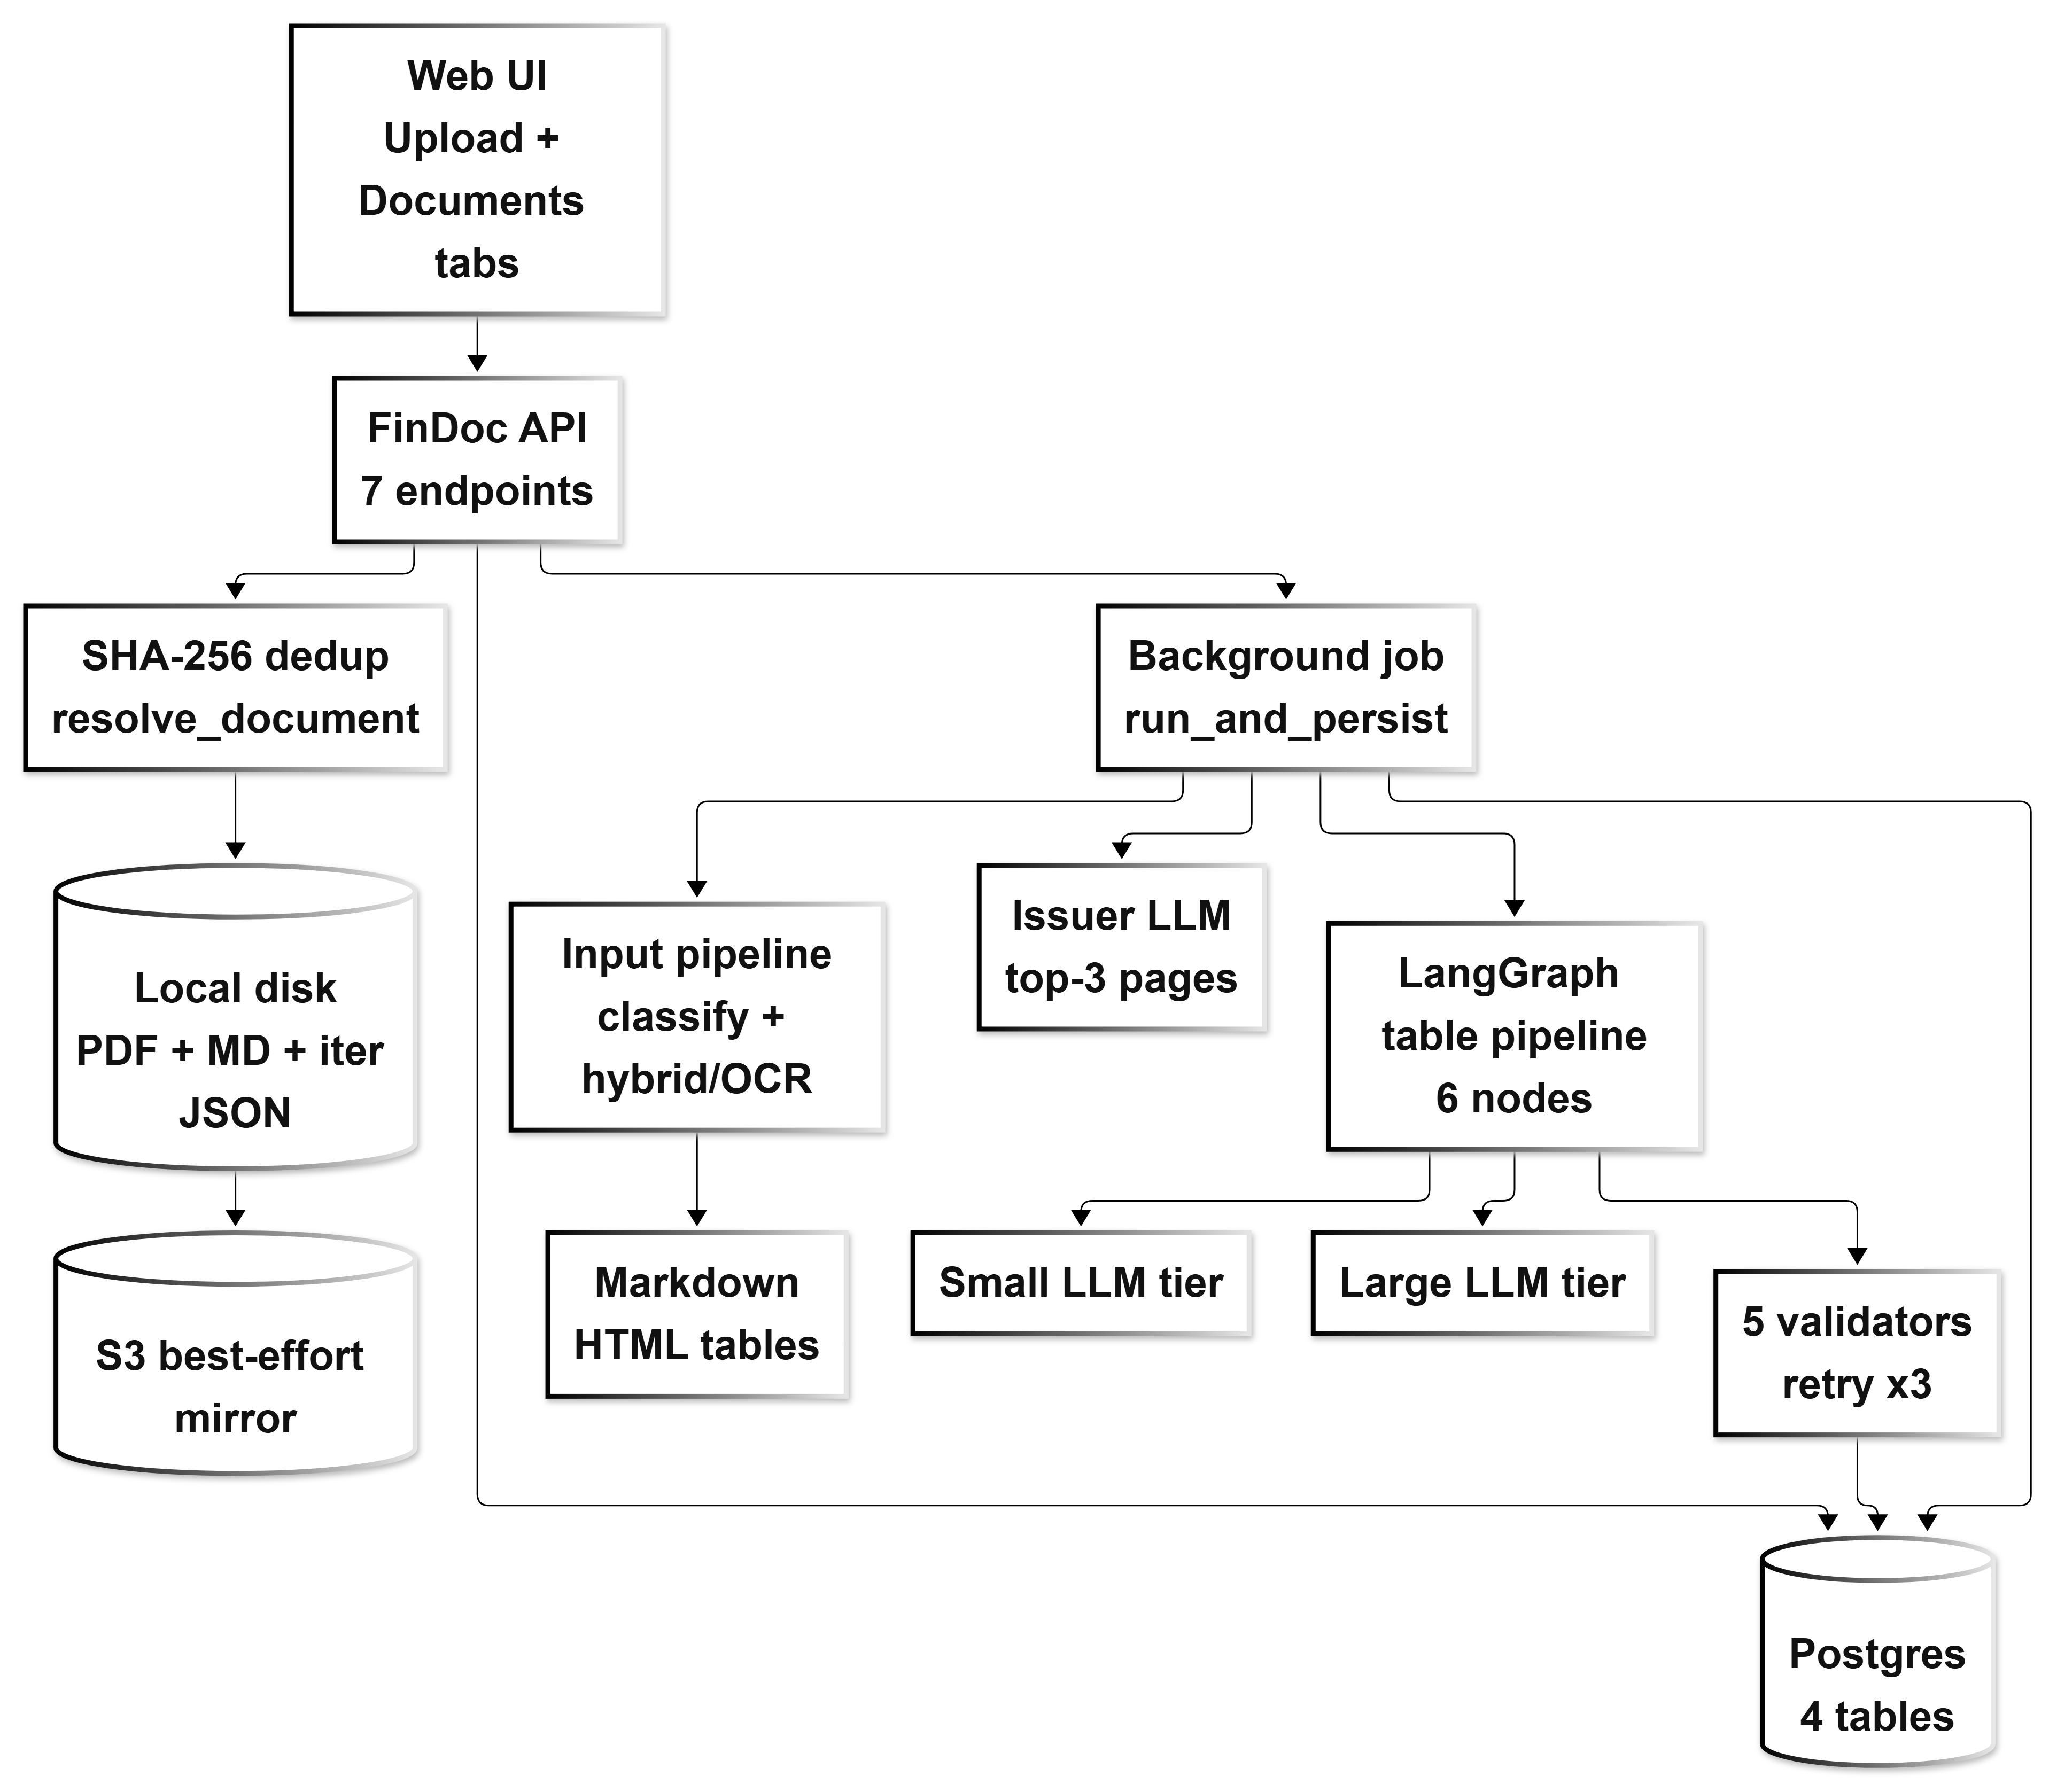
\includegraphics[width=\textwidth,height=0.85\textheight,keepaspectratio]{../diagrams/findoc_intelligence/04_flowchart_12-high-level-architecture.png}
\caption{High-Level Design}
\label{fig:ch03_findoc_data_extraction-04-flowchart-12-high-level-architecture}
\end{figure}

\speaker{Interviewer}{Why is the page index in memory?}

\speaker{Candidate}{I would use it for issuer detection only. It loads pages and embeddings for a document during processing. It is not a persistent vector database and it is not used by the table extraction agents.}

\speaker{Interviewer}{What about the \texttt{tools.py} search tools?}

\speaker{Candidate}{I would leave generic search tools out of the active path. The issuer detector would call the page index directly, and the table agents would receive Markdown and HTML tables directly. I would document that distinction to prevent an engineer from assuming a tool-calling retrieval workflow exists.}

\speaker{Interviewer}{Let us go one level deeper into the FastAPI service and pipeline modules.}

\medskip\hrule\medskip
\section{Low-Level Design}
\label{sec:ch03_findoc_data_extraction-13-low-level-design}

\subsection{FastAPI Application}

\speaker{Interviewer}{What belongs in \texttt{api/main.py}?}

\speaker{Candidate}{I would keep the FastAPI application, endpoint handlers, request and response DTOs, database initialization, and background-task scheduling together. It would be a compact service rather than a fully decomposed service.}

\speaker{Interviewer}{What coordinates document processing after the upload returns?}

\subsection{Extraction Orchestrator}

\speaker{Interviewer}{What is the role of \texttt{extraction.py}?}

\speaker{Candidate}{It coordinates document processing. It calls the input pipeline, builds the page index, detects issuer metadata, invokes the fundamentals graph, retries extraction when validation produces issues, and returns a document-level extraction result.}

\speaker{Interviewer}{Why structure the table pipeline with LangGraph?}

\subsection{LangGraph Pipeline}

\speaker{Interviewer}{Why use LangGraph for this pipeline?}

\speaker{Candidate}{The processing has explicit stages and a retry loop. LangGraph makes those nodes and state transitions visible. The graph contains table finding, relevance filtering, statement classification, consolidation classification, line-item extraction, and aggregation. The retry loop is handled around extraction and aggregation after validation.}

\speaker{Interviewer}{Is LangGraph being used as an autonomous agent with arbitrary tool use?}

\speaker{Candidate}{No. It is being used mainly as a structured workflow graph. The table nodes receive defined inputs and return structured outputs. There would be no tool-calling retrieval loop in this design.}

\speaker{Interviewer}{Why split classification and extraction across small and large models?}

\subsection{LLM Model Tiers}

\speaker{Interviewer}{Why use both a small and a large model?}

\speaker{Candidate}{Filtering and classification are relatively constrained tasks, so a smaller model can handle them more cheaply. Full table transcription requires more context and careful structured output, so the larger model is used there. This separates cost-sensitive classification from accuracy-sensitive extraction.}
\speaker{Candidate}{Can I make the tiering and cost arithmetic concrete for capacity planning?}
\speaker{Interviewer}{Yes, which models and how many calls per document?}
\speaker{Candidate}{The small tier handles relevance, statement, and consolidation classification with one call per table at each stage, while the large tier handles line-item extraction with one call per kept table per iteration and an 8192-token limit against a 4096-token base. Issuer detection adds one default-tier call per document from the top three embedded pages, and all tiers run at temperature zero for determinism. Per document the expected LLM calls are roughly one issuer call plus one call per raw table plus one per relevant table plus one per classified table plus kept tables times iterations, where iterations range from 1 to 3. For the business this formula turns table counts into a cost and latency forecast before upload, and explains why freezing classification during retry matters: it bounds the expensive large-model calls.}
\speaker{Interviewer}{How do you enforce structured outputs from the table agents?}

\subsection{Structured Outputs}

\speaker{Interviewer}{How do you prevent the model from returning arbitrary prose?}

\speaker{Candidate}{The table agents use structured-output schemas through function-calling. For example, relevance returns \texttt{RelevanceVerdict}, statement classification returns \texttt{StatementClassification}, consolidation returns \texttt{ConsolidationMeta}, and extraction returns \texttt{ExtractedLineItems}. If the model cannot produce a valid structured object, the table can be dropped or the pipeline can record a diagnostic.}

\speaker{Candidate}{The pipeline design is complete. Shall we stress-test edge cases and failures?}

\medskip\hrule\medskip
\section{Edge Cases and Failure Scenarios}
\label{sec:ch03_findoc_data_extraction-14-edge-cases-and-failure-scenarios}

\speaker{Interviewer}{Let us stress test the design.}

\subsection{Case 1: Missing Project Name}

\speaker{Interviewer}{The user uploads a file but does not provide \texttt{project\_name}. What happens?}

\speaker{Candidate}{The API returns a validation error because \texttt{project\_name} is a required form field. The upload should not create a project.}

\subsection{Case 2: No Files}

\speaker{Interviewer}{What if the request contains a project name but no files?}

\speaker{Candidate}{The HTTP layer allows it. The project can be created and completed with zero documents because files are optional at transport level. From a product perspective, it is not useful, so the UI should ideally require at least one file.}

\subsection{Case 3: XBRL Upload}

\speaker{Interviewer}{What if the user uploads an XBRL file?}

\speaker{Candidate}{The classifier detects XBRL from the extension or content markers and rejects it as unsupported. The user should convert it to PDF for this version.}

\subsection{Case 4: Image-Only PDF}

\speaker{Interviewer}{What if the PDF has no text layer?}

\speaker{Candidate}{The classifier marks it as scanned and attempts OCR. If OCR produces usable Markdown, the pipeline continues. If no usable content is produced, the document receives a diagnostic and no downstream extraction is attempted.}

\subsection{Case 5: Narrative-Only Report}

\speaker{Interviewer}{What if a report has no financial tables?}

\speaker{Candidate}{Table discovery returns zero candidates. The document can still be stored and the project can complete with zero line items. This is different from a processing failure.}

\subsection{Case 6: OCR-Merged Cell}

\speaker{Interviewer}{OCR merges two values into one cell. How do you handle it?}

\speaker{Candidate}{The table post-processor identifies common pipe-separated merged values, repairs the HTML grid, and normalizes header spans before the LLM receives the table. Remaining issues may be detected by validation or appear in the final validation flags.}

\subsection{Case 7: Conflicting Duplicate Label}

\speaker{Interviewer}{The same label appears twice for the same period and section but has different values. What happens?}

\speaker{Candidate}{The ambiguous-duplicate-label validator records an error. The issue is attributed to the source table where possible, correction notes are generated, and extraction retries up to the third iteration. If the conflict remains, both surviving data and the validation error are persisted.}

\subsection{Case 8: Re-upload with a New Filename}

\speaker{Interviewer}{The user uploads identical PDF bytes under another filename. What happens?}

\speaker{Candidate}{SHA-256 resolution finds the existing document. The first filename remains the canonical filename, and the new project links to the existing document record.}

\subsection{Case 9: S3 Failure}

\speaker{Interviewer}{What if S3 or ADLS is unavailable during upload?}

\speaker{Candidate}{The upload must fail clearly with a retryable error. Since the object store is authoritative, the API should not accept a project it cannot persist. The failure is recorded and the client retries with backoff.}

\subsection{Case 10: Database Failure During Finalization}

\speaker{Interviewer}{What if one document is processed successfully but the final project commit fails?}

\speaker{Candidate}{The transaction should roll back the batch changes. The project is then marked failed in a separate recovery path. This preserves atomic behavior, although a production system could use per-document commits and resumable job states if larger batches become common.}

\subsection{Case 11: Background Process Crash}

\speaker{Interviewer}{What if the FastAPI process crashes during background extraction?}

\speaker{Candidate}{Because \texttt{BackgroundTasks} is in-process, the job may be lost. The database may remain in \texttt{processing}. I would accept this trade-off for the first version. For production scale, I would add a durable queue, idempotent job records, leases, and recovery for abandoned jobs.}

\subsection{Case 12: Different Projects Need Different Results}

\speaker{Interviewer}{Suppose the same document is processed in two projects with different instructions. Can this data model support that?}

\speaker{Candidate}{Not safely. Since line items are scoped to \texttt{document\_id}, reprocessing replaces the shared document's line items. A future version should introduce \texttt{document\_versions} or project-scoped extraction runs so each run has independent outputs.}
\subsection{Case 13: Concurrent Identical Uploads}
\speaker{Candidate}{Before closing edge cases, can I add two additional failure modes?}
\speaker{Interviewer}{Go ahead. What happens when two users upload identical bytes at the same time?}
\speaker{Candidate}{Both requests compute the same content hash and race to insert the same document row, so one can hit a unique-constraint violation on the hash. For the analyst this looks like a random upload failure for a file that should deduplicate cleanly. The fix is to handle the integrity error by re-reading the winner row and linking to it, or to serialize inserts on the hash, so concurrent deduplication converges instead of erroring.}
\subsection{Case 14: Zero Line Items Versus Failure}
\speaker{Interviewer}{And how does the analyst tell a still-processing document from a failed one?}
\speaker{Candidate}{Today they cannot do it reliably from counts alone, because a document list with zero line items conflates processing with failure. There is no per-document status; only the project carries processing, completed, or failed. For the business this means support cannot answer whether to wait or re-upload. The remedy is a per-document status with timestamps and diagnostics, so the Documents tab can distinguish queued, extracting, completed-empty, and failed states.}
\speaker{Candidate}{Edge cases are covered. Shall we define how to evaluate extraction quality?}

\medskip\hrule\medskip
\section{Evaluation Framework}
\label{sec:ch03_findoc_data_extraction-15-evaluation-framework}

\speaker{Interviewer}{How would you evaluate the complete pipeline?}

\speaker{Candidate}{I would build a golden dataset containing annual reports, quarterly reports, scanned documents, image-heavy tables, multi-level headers, consolidated and standalone columns, multiple currencies, negative values, duplicate labels, and tables with no relevant financial data.}

\speakcont{For each document, human annotators would label:}

\begin{itemize}[leftmargin=\speakwid]
\item Relevant tables.
\item Statement type.
\item Consolidated columns.
\item Segment context.
\item Every expected line item.
\item Period and period type.
\item Currency and scale.
\item Expected sign.
\item Source page.
\item Acceptable validation warnings.
\end{itemize}
\speakcont{Then I would evaluate each pipeline stage separately.}

\begin{xltabular}{\textwidth}{>{\raggedright\arraybackslash}X >{\raggedright\arraybackslash}X}
\caption{Evaluation Framework}\label{tab:ch03_findoc_data_extraction-15-evaluation-framework-4}\\
\hline
\textbf{Stage} & \textbf{Metrics} \\
\hline
\endfirsthead
\caption[]{Evaluation Framework (continued)}\\
\hline
\textbf{Stage} & \textbf{Metrics} \\
\hline
\endhead
PDF classification & Class accuracy, false rejection rate \\
Markdown and table conversion & Table recall, malformed-table rate \\
Relevance filtering & Precision, recall, F1 \\
Statement classification & Accuracy and confusion matrix \\
Consolidation classification & Column-selection accuracy \\
Line-item extraction & Field-level precision, recall, exact-match rate \\
Validation & Issue detection precision and recall \\
Retry loop & Resolution rate by iteration \\
Persistence & Record completeness and lineage correctness \\
End-to-end & Successful completion, latency, analyst time saved \\
\hline
\end{xltabular}

\speaker{Interviewer}{How would you evaluate LLM extraction beyond exact string matching?}

\speaker{Candidate}{I would compare normalized semantic fields. For example, ``Total assets'' and ``Total assets$^1$'' may be the same label after footnote cleanup. Numeric comparison should use tolerance where appropriate, while period, sign, consolidation status, and source page should be evaluated exactly or with clearly defined rules.}

\speaker{Interviewer}{Before production in a bank, what security and hardening concerns remain?}

\medskip\hrule\medskip
\section{Security and Production Hardening}
\label{sec:ch03_findoc_data_extraction-16-security-and-production-hardening}

\speaker{Interviewer}{What production concerns would you address before deploying this to a bank or investment firm?}

\speaker{Candidate}{I would address the following:}

\begin{itemize}[leftmargin=\speakwid]
\item Add authentication and authorization; the \texttt{requested\_by} value is free text and is not an identity boundary.
\item Validate filename handling and prevent path traversal.
\item Enforce upload-size limits in the actual request path.
\item Scan uploads for malware.
\item Encrypt files at rest and in transit.
\item Use object storage as the durable source before running multiple replicas.
\item Avoid logging sensitive document content or LLM prompts.
\item Add structured audit logs for extraction and validation decisions.
\item Add rate limits and model-cost controls.
\item Protect the LLM endpoint and secrets.
\item Add durable job execution and retry policies.
\item Add database indexes for common document and line-item queries.
\item Add observability for latency, token usage, OCR failures, and validator outcomes.
\end{itemize}

\speaker{Interviewer}{To avoid confusion, what is explicitly out of scope for this version?}

\medskip\hrule\medskip
\section{Known Scope Boundaries}
\label{sec:ch03_findoc_data_extraction-17-known-scope-boundaries}

\speaker{Interviewer}{What would you explicitly tell stakeholders is not implemented?}

\speaker{Candidate}{I would be very direct:}

\begin{itemize}[leftmargin=\speakwid]
\item No ratio calculation.
\item No financial trend analytics.
\item No credit-risk scorecard.
\item No probability of default, LGD, or expected loss.
\item No investment recommendation.
\item No web or news search.
\item No sentiment analysis.
\item No yfinance backfill.
\item No human review or correction API.
\item No rerun endpoint.
\item No persistent vector database for table retrieval.
\item No active tool-calling extraction agents.
\item No durable external job queue.
\item No warehouse or cross-document analytics layer.
\end{itemize}
\speakcont{These are possible future capabilities, but they should not be described as current behavior.}

\speaker{Candidate}{Scope boundaries are clear. Shall I summarize the final design?}

\medskip\hrule\medskip
\section{Final Interview Discussion}
\label{sec:ch03_findoc_data_extraction-18-final-interview-discussion}

\speaker{Interviewer}{Give me the final design in a few sentences.}

\speaker{Candidate}{I would build a single FastAPI financial-document extraction service. The API quickly accepts a project and PDFs, uses SHA-256 to deduplicate documents, stores the initial project state, and schedules background processing. The pipeline classifies the input, converts PDF pages into Markdown with HTML tables, detects issuer metadata, discovers and filters relevant tables, classifies statements and consolidated columns, extracts flattened line items with structured LLM outputs, validates them deterministically, retries extraction up to three times, and persists surviving facts with source and validation metadata. The UI polls project status and lets analysts browse processed documents and grouped line items.}

\speakcont{The design deliberately keeps the LLM's role narrow and auditable. It classifies and transcribes; Python validates, retries, stores, and exposes the data. That gives the first release a realistic scope, a clear data contract, and a path to add ratios, research, or risk analytics later without pretending those features already exist.}

\speaker{Interviewer}{Good. That is a practical design because you clarified the business problem, separated current scope from future vision, and explained the design and trade-offs instead of jumping directly to technology names.}

\section*{Source Code}

The complete implementation for the Financial Document Data Extraction Agent is available in the accompanying GitHub repository:

\begin{center}
\url{https://github.com/GSaiDheeraj/Finance-and-Banking-AI-Usecases/tree/main/FinDoc_Intelligence_Agent}
\end{center}
